\chapter{Evaluation}
\definecolor{green}{RGB}{0,153,0}
The design of each strategy and the backtesting system allows for extensive parameterisation, providing multiple axes for analysis. Parameters that can be adjusted are at what number of standard deviations away from the mean spread a threshold should be set and a signal to be generated, how the trades are executed, limits on how much gas price should be when executing a trade, and also the volume of the initial investment. These are all factors that can affect the returns of the trading strategy. In the following sections, we will examine the performance of the strategy by varying these parameters, providing valuable insights into their influence on trading outcomes. For the purpose of data visualisation, we denote the liquidity pool pairs by their index; see Table \ref{tab:pool-labels}. Note that \textcolor{red}{-100\%} in the tables below indicate one of the token's balance in the account falls below 0, resulting in bankruptcy.
\begin{table}[!ht]
    \centering
    \begin{adjustwidth}{-0.5in}{-0.9in}
        \begin{tabular}{|p{20em}|p{20em}|p{3em}|}\hline
            Pool1 & Pool2 & Label\\\hline
            \truncate{20em}{USDC\_WETH\_0x88e6a0c2ddd26feeb64f039a2c41296fcb3f5640} & \truncate{20em}{USDC\_WETH\_0xe0554a476a092703abdb3ef35c80e0d76d32939f} & 0\\\hline
            \truncate{20em}{USDC\_WETH\_0x8ad599c3a0ff1de082011efddc58f1908eb6e6d8} & \truncate{20em}{USDC\_WETH\_0xe0554a476a092703abdb3ef35c80e0d76d32939f} & 1\\\hline
            \truncate{20em}{WETH\_USDT\_0x11b815efb8f581194ae79006d24e0d814b7697f6} & \truncate{20em}{USDC\_WETH\_0xe0554a476a092703abdb3ef35c80e0d76d32939f} & 2\\\hline
            \truncate{20em}{WETH\_USDT\_0x4e68ccd3e89f51c3074ca5072bbac773960dfa36} & \truncate{20em}{USDC\_WETH\_0xe0554a476a092703abdb3ef35c80e0d76d32939f} & 3\\\hline
            \truncate{20em}{DAI\_WETH\_0x60594a405d53811d3bc4766596efd80fd545a270} & \truncate{20em}{USDC\_WETH\_0xe0554a476a092703abdb3ef35c80e0d76d32939f} & 4\\\hline
            \truncate{20em}{DAI\_WETH\_0xc2e9f25be6257c210d7adf0d4cd6e3e881ba25f8} & \truncate{20em}{USDC\_WETH\_0xe0554a476a092703abdb3ef35c80e0d76d32939f} & 5\\\hline
            \truncate{20em}{USDC\_WETH\_0xe0554a476a092703abdb3ef35c80e0d76d32939f} & \truncate{20em}{WETH\_USDT\_0xc5af84701f98fa483ece78af83f11b6c38aca71d} & 6\\\hline
        \end{tabular}
    \end{adjustwidth}
    \caption{Liquidity pool pairs and their corresponding labels \label{tab:pool-labels}}
\end{table}
\vspace{-4ex}
\section{Trading System}
The implemented backtesting system is designed to be robust and comprehensive, taking into account all the necessary costs associated with trading, as discussed in Section \ref{sec:backtesting-sys}. However, there are a couple of areas that could benefit from further improvement.
\\[3mm]
One aspect that could be enhanced is the data granularity of the pricing data used in the backtesting system. Currently, the system utilises hourly data points, which may not capture all the nuances and intraday price movements. By incorporating more granular data, such as minute-by-minute or even tick-level data, the system could provide a more accurate representation of market dynamics and potentially improve the accuracy of the backtest results.
\\[3mm]
Additionally, when executing swaps or trades, it is important to consider the impact of slippage. Slippage refers to the price difference that occurs when executing a trade due to changes in the market conditions, such as supply differences between trading pairs. To account for slippage, the system should incorporate realistic price adjustments to accurately simulate the trading environment. This can help ensure that the backtest results reflect the actual performance that would be achieved in real trading scenarios. However, this is somewhat mitigated as only larger liquidity pools, with a volume of $\geq \$10 million$, are used and with only a maximum of 100ETH (\$394,626.00) being traded in each pool, the effects of slippage become very small in such scenarios.
\\[3mm]
By addressing these aspects and refining the data granularity, and furthering the slippage considerations, the backtesting system can provide more precise and reliable results, leading to improved insights into the profitability and viability of the trading strategy under evaluation.

\section{Strategy Parameters}
\label{sec:strat-param}

\subsection{Number of Standard Deviations away from the mean}
Varying the standard deviation in a mean reversion pairs trading strategy can have a significant impact on the strategy's returns. When the number of standard deviations is set too high, it means that the spread between the pair's prices must deviate significantly from the mean before a signal is generated. In this case, the strategy may generate fewer trades, resulting in longer holding periods for positions; however, this tends to have a greater return per trade. On the other hand, setting a lower number of standard deviations makes the strategy more sensitive to smaller deviations from the mean. This increases the frequency of trade signals and potentially leads to more active trading. However, it also exposes the strategy to a higher risk of false signals or trading on noise in the price data. It can result in higher transaction costs and potentially lower returns due to increased trading activity, potentially resulting in losses. For the purpose of simplicity, $\#_{\sigma}$ denotes this parameter.
\\[3mm]
Table \ref{tab:varying_sigma} displays the returns as the standard deviations away from the mean the threshold is set. For the purpose of this experiment, the other parameters were; 100 ETH worth of initial investment, the window size set to 30 days, a gas price threshold of 1 ETH (i.e. not having a threshold), the interactions with the blockchain to be separately executed and finally the lag that the lagged strategy uses are set to 1 hour. The period that trading occurs is from 18th December 2021 to 9th June 2023.
\\[3mm]
We can see that as $\#_{\sigma} \rightarrow 0$, the number of trades increases; however, this causes the returns to be more negative (and in some cases terminating early with 100\% loss) than positive, likely due to trades being opened when gas fees are substantially larger than the profit. However, if $\#_{\sigma}$ is larger, although the profits from each trade increase, the number of opportunities that were actionable were limited. Another interesting feature that can easily be spotted is that the Constant Hedge Ratio Strategy makes little to no profit in all cases, whereas the other strategies perform better as $\#_{\sigma} \rightarrow \sim 1.75$. Furthermore, all of the strategies return a profit on pool pair 6 with the exception of the Kalman Filter Strategy, albeit with a higher threshold.
\\[3mm]
Consistent profit among all of the pool pairs, excluding pool pair 6, is also achieved at different numbers of standard deviations. We can see in Figure \ref{fig:varyStd} that the average return across all liquidity pool pairs that each strategy generates at each standard deviation. The Kalman Filter becomes largely profitable at $\#_{\sigma} = 0.5$, whereas the lagged and sliding window strategies become profitable at $\#_{\sigma} = 2$. The reason for this is highly due to the fact that the Kalman Filter and the Granger Causality tests are better able to find underlying trends, thus being better at selecting the hedge ratio, which in turn affects the volumes being traded and hence the effect of the returns.

\begin{table}[!htb]
    \centering
    \begin{adjustwidth}{-0.8in}{-0.9in}
        \begin{tabular}{|p{4em}|p{2em}|p{3em}|p{3em}|p{3em}|p{3em}|p{3em}|p{3em}|p{3em}|p{3em}|p{3em}|p{3em}|}\hline
            Std & Pool Pair & \multicolumn{10}{|c|}{Strategy's Annual Percentage Rate (APR) - Trading from 18th December 2021 to 9th June 2023} \\\cline{3-12}
            &   & \multicolumn{2}{|c|}{Constant} & \multicolumn{2}{|c|}{Sliding Window} & \multicolumn{2}{|c|}{Lagged} & \multicolumn{2}{|c|}{Granger Causality} & \multicolumn{2}{|c|}{Kalman Filter}\\\cline{3-12}
            & & Return \% & \# of Trades & Return \% & \# of Trades & Return \% & \# of Trades & Return \% & \# of Trades & Return \% & \# of Trades\\\hline

            & 0 & \textcolor{green}{3.66} & 360 & \textcolor{green}{19.02} & 661 & \textcolor{green}{41.18} & 687 & \textcolor{green}{17.8} & 275 & \textcolor{green}{50.66} & 228\\\cline{3-12}
            & 1 & \textcolor{red}{-41.23} & 397 & \textcolor{red}{-70.78} & 660 & \textcolor{red}{-63.39} & 653 & \textcolor{red}{-40.2} & 388 & \textcolor{red}{-10.43} & 307\\\cline{3-12}
            & 2 & \textcolor{green}{3.92} & 454 & \textcolor{red}{-1.43} & 634 & \textcolor{green}{27.81} & 619 & \textcolor{green}{24.64} & 300 & \textcolor{green}{54.06} & 236\\\cline{3-12}
            $\#_{\sigma}=0.1$ & 3 & \textcolor{red}{-53.35} & 535 & \textcolor{red}{-56.31} & 572 & \textcolor{red}{-59.1} & 604 & \textcolor{red}{-33.24} & 375 & \textcolor{red}{-9.76} & 301\\\cline{3-12}
            & 4 & \textcolor{green}{7.42} & 375 & \textcolor{green}{6.72} & 759 & \textcolor{green}{36.73} & 669 & \textcolor{green}{16.18} & 296 & \textcolor{green}{44.35} & 227\\\cline{3-12}
            & 5 & \textcolor{red}{-40.45} & 396 & \textcolor{red}{-61.12} & 587 & \textcolor{red}{-54.1} & 593 & \textcolor{red}{-37.0} & 337 & \textcolor{red}{-17.72} & 328\\\cline{3-12}
            & 6 & \textcolor{red}{-11.0} & 72 & \textcolor{red}{-68.8} & 213 & \textcolor{red}{-62.28} & 198 & \textcolor{red}{-13.58} & 68 & \textcolor{red}{-4.2} & 84\\\hline\hline

            & 0 & \textcolor{green}{7.84} & 723 & \textcolor{red}{-11.01} & 1223 & \textcolor{green}{62.43} & 1185 & \textcolor{green}{66.93} & 550 & \textcolor{green}{130.2} & 378\\\cline{3-12}
            & 1 & \textcolor{red}{-100.0} & 832 & \textcolor{red}{-100.0} & 920 & \textcolor{red}{-100.0} & 936 & \textcolor{red}{-56.1} & 650 & \textcolor{green}{39.26} & 456\\\cline{3-12}
            & 2 & \textcolor{green}{6.14} & 688 & \textcolor{red}{-0.59} & 1105 & \textcolor{green}{73.22} & 1025 & \textcolor{green}{71.64} & 630 & \textcolor{green}{153.85} & 396\\\cline{3-12}
            $\#_{\sigma}=0.5$ & 3 & \textcolor{red}{-84.34} & 794 & \textcolor{red}{-100.0} & 944 & \textcolor{red}{-82.5} & 1063 & \textcolor{red}{-51.1} & 691 & \textcolor{green}{24.18} & 425\\\cline{3-12}
            & 4 & \textcolor{green}{16.97} & 826 & \textcolor{red}{-11.24} & 1243 & \textcolor{green}{66.69} & 1213 & \textcolor{green}{47.5} & 538 & \textcolor{green}{131.36} & 391\\\cline{3-12}
            & 5 & \textcolor{red}{-86.92} & 837 & \textcolor{red}{-100.0} & 854 & \textcolor{red}{-100.0} & 905 & \textcolor{red}{-24.3} & 503 & \textcolor{green}{54.86} & 388\\\cline{3-12}
            & 6 & \textcolor{red}{-27.3} & 124 & \textcolor{red}{-90.13} & 359 & \textcolor{red}{-71.37} & 301 & \textcolor{red}{-3.33} & 56 & \textcolor{red}{-29.04} & 150\\\hline\hline
            
            & 0 & \textcolor{red}{-15.08} & 675 & \textcolor{red}{-1.08} & 864 & \textcolor{green}{75.76} & 865 & \textcolor{green}{60.3} & 586 & \textcolor{green}{93.32} & 442\\\cline{3-12}
            & 1 & \textcolor{red}{-100.0} & 791 & \textcolor{red}{-100.0} & 814 & \textcolor{red}{-85.22} & 1022 & \textcolor{red}{-40.6} & 641 & \textcolor{red}{-7.2} & 505\\\cline{3-12}
            & 2 & \textcolor{red}{-14.94} & 535 & \textcolor{green}{4.72} & 777 & \textcolor{green}{86.24} & 721 & \textcolor{green}{75.65} & 497 & \textcolor{green}{103.11} & 404\\\cline{3-12}
            $\#_{\sigma}=1$ & 3 & \textcolor{red}{-100.0} & 497 & \textcolor{red}{-100.0} & 657 & \textcolor{red}{-64.55} & 872 & \textcolor{red}{-26.11} & 550 & \textcolor{green}{1.42} & 436\\\cline{3-12}
            & 4 & \textcolor{red}{-3.6} & 689 & \textcolor{green}{10.29} & 799 & \textcolor{green}{89.18} & 822 & \textcolor{green}{74.11} & 558 & \textcolor{green}{105.91} & 460\\\cline{3-12}
            & 5 & \textcolor{red}{-100.0} & 533 & \textcolor{red}{-100.0} & 612 & \textcolor{red}{-58.88} & 785 & \textcolor{red}{-25.29} & 500 & \textcolor{green}{26.89} & 408\\\cline{3-12}
            & 6 & \textcolor{red}{-40.18} & 108 & \textcolor{red}{-52.01} & 169 & \textcolor{red}{-34.85} & 125 & \textcolor{red}{-21.08} & 70 & \textcolor{red}{-30.59} & 158\\\hline\hline
            
            & 0 & \textcolor{green}{3.83} & 365 & \textcolor{green}{30.85} & 447 & \textcolor{green}{83.24} & 476 & \textcolor{green}{79.52} & 272 & \textcolor{green}{100.22} & 179\\\cline{3-12}
            & 1 & \textcolor{red}{-100.0} & 408 & \textcolor{red}{-53.49} & 509 & \textcolor{red}{-23.97} & 504 & \textcolor{green}{7.18} & 293 & \textcolor{green}{48.04} & 221\\\cline{3-12}
            & 2 & \textcolor{red}{-4.17} & 302 & \textcolor{green}{14.67} & 402 & \textcolor{green}{68.45} & 391 & \textcolor{green}{79.98} & 250 & \textcolor{green}{96.97} & 147\\\cline{3-12}
            $\#_{\sigma}=1.5$ & 3 & \textcolor{red}{-57.3} & 389 & \textcolor{red}{-44.96} & 453 & \textcolor{red}{-19.47} & 449 & \textcolor{green}{5.83} & 290 & \textcolor{green}{48.86} & 166\\\cline{3-12}
            & 4 & \textcolor{red}{-8.38} & 324 & \textcolor{green}{24.77} & 428 & \textcolor{green}{75.32} & 426 & \textcolor{green}{85.94} & 273 & \textcolor{green}{99.13} & 201\\\cline{3-12}
            & 5 & \textcolor{red}{-100.0} & 312 & \textcolor{red}{-42.04} & 402 & \textcolor{red}{-2.13} & 379 & \textcolor{green}{23.05} & 259 & \textcolor{green}{60.87} & 175\\\cline{3-12}
            & 6 & \textcolor{red}{-31.39} & 77 & \textcolor{red}{-29.45} & 87 & \textcolor{red}{-29.0} & 89 & \textcolor{red}{-13.84} & 35 & \textcolor{red}{-12.98} & 102\\\hline\hline
            
            & 0 & \textcolor{red}{-7.14} & 288 & \textcolor{green}{24.57} & 342 & \textcolor{green}{81.97} & 353 & \textcolor{green}{61.58} & 192 & \textcolor{green}{98.76} & 153\\\cline{3-12}
            & 1 & \textcolor{red}{-52.98} & 358 & \textcolor{red}{-20.9} & 293 & \textcolor{red}{-5.29} & 323 & \textcolor{green}{12.99} & 213 & \textcolor{green}{45.66} & 178\\\cline{3-12}
            & 2 & \textcolor{red}{-1.71} & 225 & \textcolor{green}{21.43} & 277 & \textcolor{green}{68.39} & 270 & \textcolor{green}{68.62} & 180 & \textcolor{green}{95.11} & 133\\\cline{3-12}
            $\#_{\sigma}=1.75$ & 3 & \textcolor{red}{-45.93} & 309 & \textcolor{red}{-14.98} & 268 & \textcolor{red}{-1.01} & 294 & \textcolor{green}{22.19} & 211 & \textcolor{green}{53.56} & 145\\[-3ex]\cline{3-12}
            & 4 & \textcolor{red}{-2.54} & 241 & \textcolor{green}{26.46} & 294 & \textcolor{green}{55.77} & 291 & \textcolor{green}{65.92} & 201 & \textcolor{green}{84.62} & 152\\\cline{3-12}
            & 5 & \textcolor{red}{-41.71} & 287 & \textcolor{red}{-9.73} & 225 & \textcolor{green}{9.79} & 250 & \textcolor{green}{20.48} & 200 & \textcolor{green}{61.97} & 152\\\cline{3-12}
            & 6 & \textcolor{red}{-35.28} & 76 & \textcolor{red}{-19.16} & 67 & \textcolor{red}{-29.96} & 76 & \textcolor{red}{-23.36} & 37 & \textcolor{red}{-16.02} & 74\\\hline\hline
            
            & 0 & \textcolor{green}{1.43} & 226 & \textcolor{green}{28.09} & 271 & \textcolor{green}{54.88} & 268 & \textcolor{green}{35.91} & 141 & \textcolor{green}{64.38} & 116\\\cline{3-12}
            & 1 & \textcolor{red}{-30.57} & 245 & \textcolor{green}{5.14} & 165 & \textcolor{green}{19.55} & 184 & \textcolor{green}{4.65} & 144 & \textcolor{green}{35.95} & 125\\\cline{3-12}
            & 2 & \textcolor{red}{-5.94} & 191 & \textcolor{green}{28.81} & 190 & \textcolor{green}{54.98} & 202 & \textcolor{green}{49.3} & 144 & \textcolor{green}{58.95} & 106\\\cline{3-12}
            $\#_{\sigma}=2$ & 3 & \textcolor{red}{-36.5} & 228 & \textcolor{green}{3.9} & 160 & \textcolor{green}{16.28} & 178 & \textcolor{green}{21.79} & 154 & \textcolor{green}{36.32} & 121\\\cline{3-12}
            & 4 & \textcolor{green}{5.85} & 206 & \textcolor{green}{29.2} & 190 & \textcolor{green}{51.79} & 201 & \textcolor{green}{46.95} & 149 & \textcolor{green}{58.28} & 125\\\cline{3-12}
            & 5 & \textcolor{red}{-19.82} & 192 & \textcolor{green}{7.19} & 138 & \textcolor{green}{21.28} & 147 & \textcolor{green}{12.38} & 138 & \textcolor{green}{42.87} & 125\\\cline{3-12}
            & 6 & \textcolor{red}{-27.18} & 65 & \textcolor{red}{-15.52} & 49 & \textcolor{red}{-17.7} & 54 & \textcolor{red}{-24.53} & 31 & \textcolor{green}{0.67} & 53\\\hline\hline

            
            & 0 & \textcolor{green}{1.75} & 54 & \textcolor{green}{18.68} & 102 & \textcolor{green}{17.31} & 83 & \textcolor{green}{27.63} & 51 & \textcolor{green}{17.88} & 51\\\cline{3-12}
            & 1 & \textcolor{red}{-3.91} & 64 & \textcolor{green}{13.87} & 49 & \textcolor{green}{12.0} & 46 & \textcolor{green}{20.85} & 60 & \textcolor{green}{15.28} & 60\\\cline{3-12}
            & 2 & \textcolor{green}{1.32} & 61 & \textcolor{green}{13.41} & 56 & \textcolor{green}{14.79} & 64 & \textcolor{green}{23.26} & 52 & \textcolor{green}{14.02} & 52\\\cline{3-12}
            $\#_{\sigma}=3$ & 3 & \textcolor{red}{-7.05} & 73 & \textcolor{green}{8.19} & 46 & \textcolor{green}{7.33} & 48 & \textcolor{green}{17.52} & 55 & \textcolor{green}{8.29} & 58\\\cline{3-12}
            & 4 & \textcolor{green}{3.13} & 67 & \textcolor{green}{20.95} & 57 & \textcolor{green}{18.84} & 64 & \textcolor{green}{26.98} & 60 & \textcolor{green}{17.25} & 57\\\cline{3-12}
            & 5 & \textcolor{red}{-4.45} & 53 & \textcolor{green}{13.73} & 39 & \textcolor{green}{12.17} & 39 & \textcolor{green}{23.27} & 51 & \textcolor{green}{17.39} & 57\\\cline{3-12}
            & 6 & \textcolor{red}{-1.17} & 13 & \textcolor{red}{-3.24} & 20 & \textcolor{red}{-2.18} & 25 & \textcolor{green}{3.19} & 5 & \textcolor{green}{8.01} & 16\\\hline
        \end{tabular}
    \end{adjustwidth}
    \caption{Returns of various standard deviation thresholds of each strategy \label{tab:varying_sigma}}.
\end{table}

\begin{figure}[h!]
    \centering
    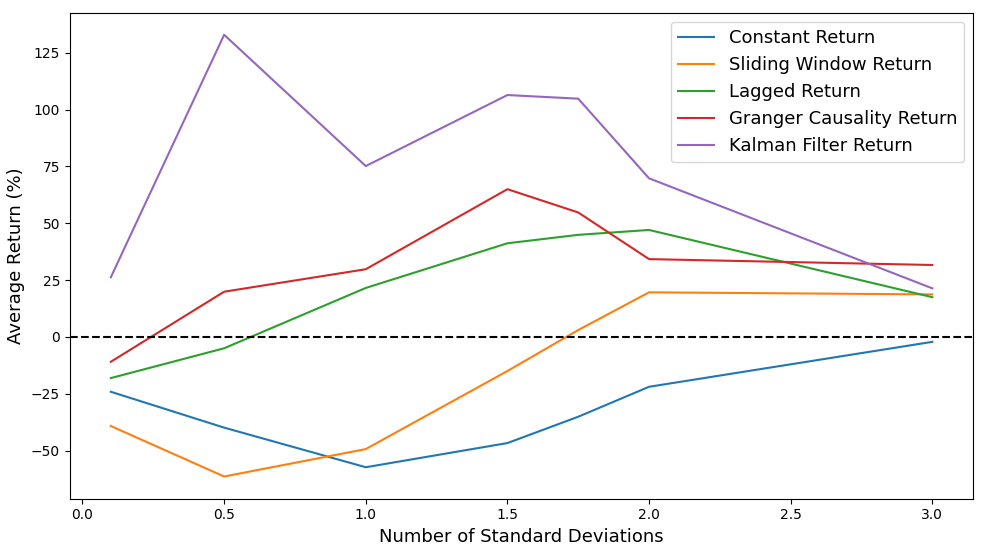
\includegraphics[width=1\textwidth]{evaluation/Images/VaryStd.png}
    \caption{Average Return across all pool pairs using various standard deviations}
    \label{fig:varyStd}
\end{figure}

\subsection{Gas Fees}
Another aspect that could be changed is fees; the first is how the transactions are executed on the blockchain and also the maximum gas price if we want to open a position. As previously mentioned, the gas fee is calculated by a combination of the gas price and the gas used. Therefore, these two parameters allow the strategy to control both the gas used and the gas price.

\subsubsection{Batched Transactions vs Separately Executed Transactions}
The method in which the transactions are executed affects how much gas is used. When transactions are executed separately, each transaction incurs its own gas cost. This means that for every individual transaction, there will be gas consumed for various operations such as contract interaction, data storage, and computational tasks. As a result, executing a large number of separate transactions can lead to a significant cumulative gas cost. On the other hand, when transactions are batched together, they are consolidated into a single transaction. This consolidation reduces the overhead associated with executing multiple transactions individually. By combining the operations of multiple transactions into a single execution, redundant computations and storage operations can be eliminated, resulting in more efficient gas usage. It can immediately be seen in Figure \ref{fig:gasResult} that the process of batching the transactions consumes less gas than the combined gas of the transactions required to execute the opening and closing of the positions.
\\[3mm]
Furthermore, the effects of using separate versus batched transactions can be seen in Table \ref{tab:BatchedVsSeperate}. The parameters used for this investigation were the same as above with the selection, e.g. $\#_{\sigma} = 1.75$, 100 ETH worth of initial investment, the window size set to 30 days, a gas price threshold of 1 ETH (i.e. not having a threshold) and the testing period remained from 18th December 2021 to 9th June 2023.

\begin{table}[H]
    \centering
    \begin{adjustwidth}{-0.8in}{-0.9in}
        \begin{tabular}{|p{2em}|p{2em}|p{3em}|p{3em}|p{3em}|p{3em}|p{3em}|p{3em}|p{3em}|p{3em}|p{3em}|p{3em}|}\hline
            & Pool Pair & \multicolumn{10}{|c|}{Strategy's Annual Percentage Rate (APR) - Trading from 18th December 2021 to 9th June 2023} \\\cline{3-12}
            &   & \multicolumn{2}{|c|}{Constant} & \multicolumn{2}{|c|}{Sliding Window} & \multicolumn{2}{|c|}{Lagged} & \multicolumn{2}{|c|}{Granger Causality} & \multicolumn{2}{|c|}{Kalman Filter}\\\cline{3-12}
            & & Return \% & \# of Trades & Return \% & \# of Trades & Return \% & \# of Trades & Return \% & \# of Trades & Return \% & \# of Trades\\\hline
            
            \parbox[t]{4em}{\multirow{7}{*}{\rotatebox[origin=c]{90}{Seperate}}} & 0 & \textcolor{red}{-7.14} & 288 & \textcolor{green}{24.57} & 342 & \textcolor{green}{81.97} & 353 & \textcolor{green}{61.58} & 192 & \textcolor{green}{98.76} & 153\\\cline{3-12}
            & 1 & \textcolor{red}{-52.98} & 358 & \textcolor{red}{-20.9} & 293 & \textcolor{red}{-5.29} & 323 & \textcolor{green}{12.99} & 213 & \textcolor{green}{45.66} & 178\\\cline{3-12}
            & 2 & \textcolor{red}{-1.71} & 225 & \textcolor{green}{21.43} & 277 & \textcolor{green}{68.39} & 270 & \textcolor{green}{68.62} & 180 & \textcolor{green}{95.11} & 133\\\cline{3-12}
            & 3 & \textcolor{red}{-45.93} & 309 & \textcolor{red}{-14.98} & 268 & \textcolor{red}{-1.01} & 294 & \textcolor{green}{22.19} & 211 & \textcolor{green}{53.56} & 145\\\cline{3-12}
            & 4 & \textcolor{red}{-2.54} & 241 & \textcolor{green}{26.46} & 294 & \textcolor{green}{55.77} & 291 & \textcolor{green}{65.92} & 201 & \textcolor{green}{84.62} & 152\\\cline{3-12}
            & 5 & \textcolor{red}{-41.71} & 287 & \textcolor{red}{-9.73} & 225 & \textcolor{green}{9.79} & 250 & \textcolor{green}{20.48} & 200 & \textcolor{green}{61.97} & 152\\\cline{3-12}
            & 6 & \textcolor{red}{-35.28} & 76 & \textcolor{red}{-19.16} & 67 & \textcolor{red}{-29.96} & 76 & \textcolor{red}{-23.36} & 37 & \textcolor{red}{-16.02} & 74\\\hline\hline

            \parbox[t]{4em}{\multirow{7}{*}{\rotatebox[origin=c]{90}{Batched}}} & 0 & \textcolor{red}{-2.2} & 288 & \textcolor{green}{30.8} & 342 & \textcolor{green}{87.79} & 353 & \textcolor{green}{66.76} & 192 & \textcolor{green}{100.13} & 153\\\cline{3-12}
            & 1 & \textcolor{red}{-47.23} & 358 & \textcolor{red}{-16.28} & 293 & \textcolor{green}{0.91} & 323 & \textcolor{green}{16.58} & 213 & \textcolor{green}{46.78} & 178\\\cline{3-12}
            & 2 & \textcolor{green}{2.63} & 225 & \textcolor{green}{28.29} & 277 & \textcolor{green}{74.07} & 270 & \textcolor{green}{75.52} & 180 & \textcolor{green}{97.43} & 133\\\cline{3-12}
            & 3 & \textcolor{red}{-42.06} & 309 & \textcolor{red}{-9.95} & 268 & \textcolor{green}{4.71} & 294 & \textcolor{green}{25.33} & 211 & \textcolor{green}{52.93} & 145\\\cline{3-12}
            & 4 & \textcolor{green}{1.72} & 241 & \textcolor{green}{29.97} & 294 & \textcolor{green}{62.84} & 291 & \textcolor{green}{69.21} & 201 & \textcolor{green}{86.18} & 152\\\cline{3-12}
            & 5 & \textcolor{red}{-37.04} & 287 & \textcolor{red}{-4.83} & 225 & \textcolor{green}{14.37} & 250 & \textcolor{green}{23.51} & 200 & \textcolor{green}{62.31} & 152\\\cline{3-12}
            & 6 & \textcolor{red}{-33.66} & 76 & \textcolor{red}{-17.93} & 67 & \textcolor{red}{-27.78} & 76 & \textcolor{red}{-21.93} & 37 & \textcolor{red}{-14.77} & 74\\\hline
        \end{tabular}
    \end{adjustwidth}
    \caption{Returns of each strategy when using seperate and batched transactions \label{tab:BatchedVsSeperate}}.
\end{table}
\noindent When comparing the use of batched transactions to executing transactions separately, it is evident that utilising batched transactions yields a higher return, as expected. The observed increase in return ranges from approximately 1\% to 8\% compared to executing the transactions individually. The higher return achieved through batched transactions can be attributed to several factors. First, as mentioned earlier, batching transactions reduces the gas costs associated with executing multiple transactions. By consolidating operations into a single transaction, redundant computations and storage operations are eliminated, resulting in more efficient gas usage. The reduction in gas costs directly contributes to the overall profitability of the trading strategy.

\subsubsection{Gas Price Threshold}
A threshold on the gas price is also set to ensure positions that have a high transaction cost associated with it are avoided. As the gas price is variable, we can see in Figure \ref{fig:GasPriceHistogram} the distribution of the gas prices over time is similar to a geometric distribution; therefore, by thresholding high gas prices, the strategies would avoid making a trade where the trade's profit would be overshadowed by the cost of trading.
\begin{figure}[h!]
    \centering
    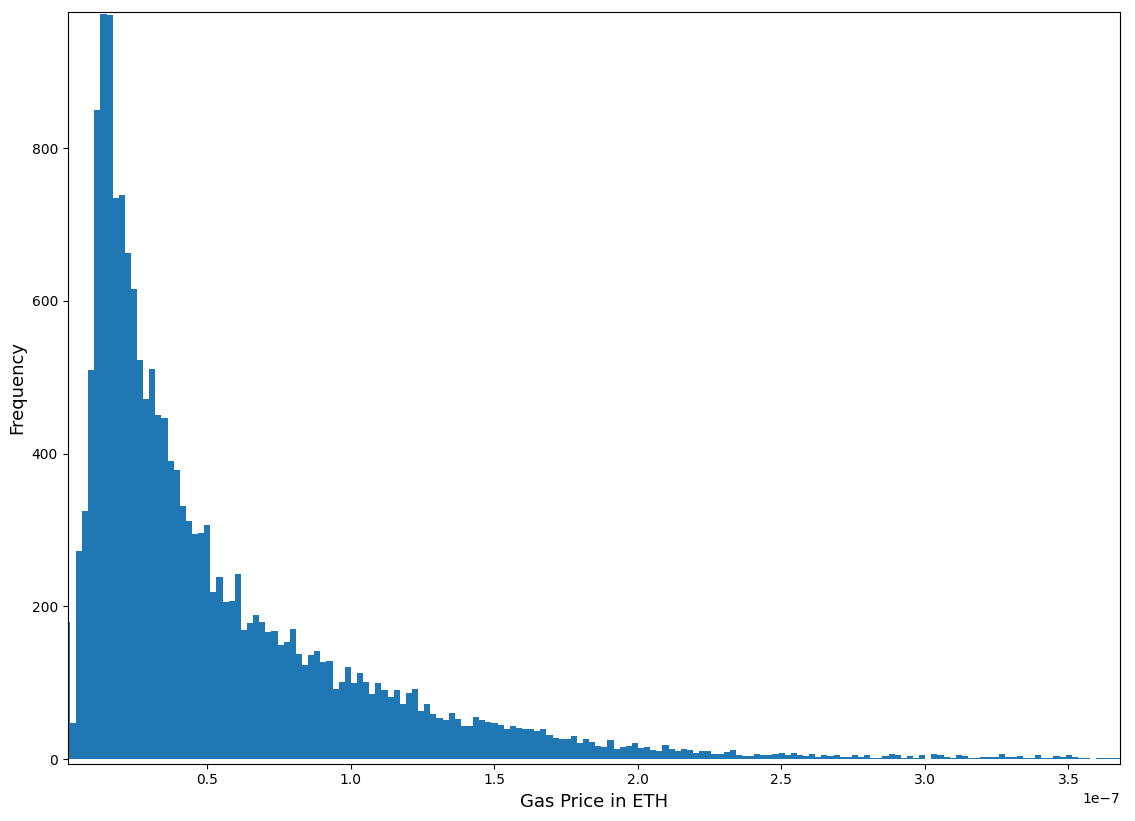
\includegraphics[width=0.7\linewidth]{evaluation/Images/GasPriceHistogram.png}
    \caption{Histogram Plot of Gas Prices in ETH}
    \label{fig:GasPriceHistogram}
\end{figure}
\\[3mm]
\noindent Therefore, our investigation consists of varying this threshold to see its effects on the returns of each strategy, using batched transactions and the same parameters used in the above experiment, the thresholds are set to the $60^{th}, 70^{th},80^{th},90^{th},100^{th}$ quantiles. Table \ref{tab:VaryGasPriceThresholds} displays the results obtained by varying these thresholds. It can be seen that filtering more costly opportunities, expectedly, reduces the number of actionable; however, the higher thresholds also show that these opportunities are still just as if not more profitable. In addition, to this, Figure \ref{fig:VaryGasPriceThresholds} shows that a low threshold benefits the constant hedge ratio strategy most as with the low threshold, it has a slight loss, and as the threshold increases, the return using the strategy decreases. Whereas the returns are hindered with a lower threshold as many profitable opportunities are missed due to the overly low threshold, resulting in a reduction in the overall profitability of the trading strategy. The figure also shows how setting the threshold after the $90^{th}$ percentile does little to no effect on the return, giving a slightly positive impact on the Lagged strategy and a slight negative impact on the remaining. This is likely due to there only a small amount of arbitrage opportunities to be present in such times when the gas price is high, thus having little impact. It is also interesting to see that the Lagged and the Kalman Filter strategies perform better by setting the threshold to the $90^{th}$ percentile in comparison to the $80^{th}$ percentile, whereas the other strategies perform worse.
\\[3mm]
Overall, the analysis of varying gas price thresholds reveals that adjusting the threshold level has a direct impact on the number of actionable opportunities and the resulting returns. Higher thresholds filter out less favourable opportunities while still maintaining profitability. However, it is crucial to strike a balance and avoid setting the threshold too low, as this may lead to missed profitable opportunities. Hence, to get the best balance, the threshold is set to the $90^{th}$ percentile.

\begin{figure}[H]
    \centering
    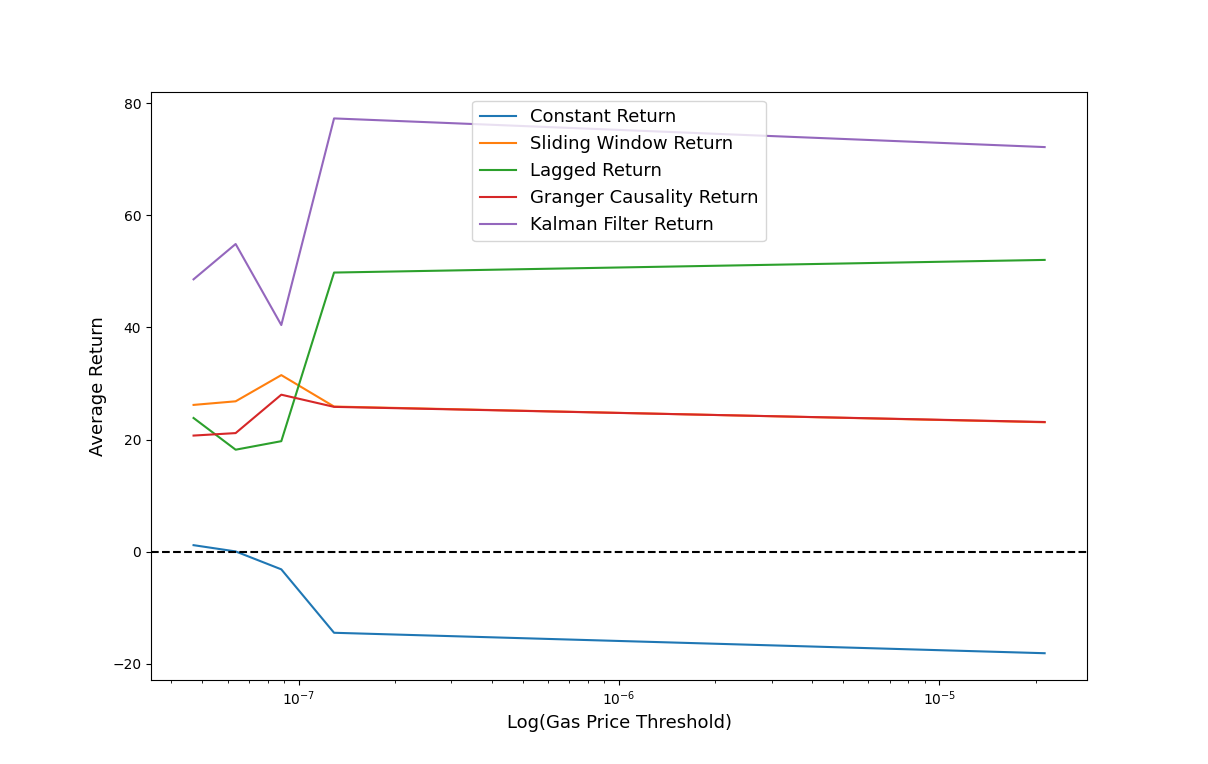
\includegraphics[width=\linewidth]{evaluation/Images/VaryGPThreshold.png}
    \caption{Average Returns of each strategy when using different gas price thresholds}
    \label{fig:VaryGasPriceThresholds}
\end{figure}

\begin{table}[htb!]
    \centering
    \begin{adjustwidth}{-0.9in}{-0.9in}
        \begin{tabular}{|p{5em}|p{2em}|p{3em}|p{3em}|p{3em}|p{3em}|p{3em}|p{3em}|p{3em}|p{3em}|p{3em}|p{3em}|}\hline
            Gas Price Threshold & Pool Pair & \multicolumn{10}{|c|}{Strategy's Annual Percentage Rate (APR) - Trading from 18th December 2021 to 9th June 2023} \\\cline{3-12}
            &   & \multicolumn{2}{|c|}{Constant} & \multicolumn{2}{|c|}{Sliding Window} & \multicolumn{2}{|c|}{Lagged} & \multicolumn{2}{|c|}{Granger Causality} & \multicolumn{2}{|c|}{Kalman Filter}\\\cline{3-12}
            & & Return \% & \# of Trades & Return \% & \# of Trades & Return \% & \# of Trades & Return \% & \# of Trades & Return \% & \# of Trades\\\hline

            & 0 & \textcolor{green}{7.97} & 193 & \textcolor{green}{26.18} & 221 & \textcolor{green}{30.36} & 242 & \textcolor{green}{30.83} & 124 & \textcolor{green}{51.35} & 105\\\cline{3-12}
            & 1 & \textcolor{red}{-23.52} & 253 & \textcolor{red}{-0.69} & 178 & \textcolor{red}{-9.49} & 205 & \textcolor{green}{7.4} & 139 & \textcolor{green}{26.12} & 124\\\cline{3-12}
            & 2 & \textcolor{green}{8.71} & 134 & \textcolor{green}{30.05} & 171 & \textcolor{green}{26.33} & 169 & \textcolor{green}{30.82} & 103 & \textcolor{green}{51.46} & 77\\\cline{3-12}
            $60^{th}$ percentile = 4.7e-08 & 3 & \textcolor{red}{-22.44} & 214 & \textcolor{green}{0.58} & 165 & \textcolor{red}{-8.34} & 188 & \textcolor{green}{7.65} & 134 & \textcolor{green}{31.41} & 90\\[-5.5ex]\cline{3-12}
            & 4 & \textcolor{green}{14.69} & 150 & \textcolor{green}{34.45} & 178 & \textcolor{green}{24.69} & 184 & \textcolor{green}{31.4} & 123 & \textcolor{green}{47.09} & 90\\\cline{3-12}
            & 5 & \textcolor{red}{-12.54} & 191 & \textcolor{green}{6.98} & 128 & \textcolor{green}{3.85} & 150 & \textcolor{green}{15.33} & 124 & \textcolor{green}{38.32} & 96\\\cline{3-12}
            & 6 & \textcolor{red}{-27.3} & 53 & \textcolor{red}{-4.83} & 30 & \textcolor{red}{-15.56} & 46 & \textcolor{red}{-25.36} & 26 & \textcolor{red}{-6.35} & 50\\\hline\hline

            & 0 & \textcolor{green}{12.85} & 216 & \textcolor{green}{33.49} & 255 & \textcolor{green}{33.74} & 277 & \textcolor{green}{33.2} & 146 & \textcolor{green}{58.28} & 120\\\cline{3-12}
            & 1 & \textcolor{red}{-24.53} & 283 & \textcolor{red}{-2.14} & 209 & \textcolor{red}{-17.44} & 243 & \textcolor{green}{4.14} & 161 & \textcolor{green}{29.83} & 140\\\cline{3-12}
            & 2 & \textcolor{green}{12.4} & 156 & \textcolor{green}{33.28} & 199 & \textcolor{green}{25.97} & 200 & \textcolor{green}{36.35} & 123 & \textcolor{green}{61.2} & 94\\\cline{3-12}
            $70^{th}$ percentile = 6.36e-08 & 3 & \textcolor{red}{-23.07} & 240 & \textcolor{green}{0.35} & 193 & \textcolor{red}{-14.67} & 219 & \textcolor{green}{4.35} & 162 & \textcolor{green}{35.85} & 107\\[-5.5ex]\cline{3-12}
            & 4 & \textcolor{green}{14.6} & 175 & \textcolor{green}{33.64} & 215 & \textcolor{green}{23.48} & 219 & \textcolor{green}{38.4} & 152 & \textcolor{green}{59.88} & 111\\\cline{3-12}
            & 5 & \textcolor{red}{-13.43} & 220 & \textcolor{green}{6.63} & 152 & \textcolor{red}{-3.77} & 179 & \textcolor{green}{13.97} & 148 & \textcolor{green}{42.8} & 116\\\cline{3-12}
            & 6 & \textcolor{red}{-26.12} & 59 & \textcolor{red}{-6.02} & 37 & \textcolor{red}{-17.86} & 56 & \textcolor{red}{-17.84} & 30 & \textcolor{red}{-8.94} & 58\\\hline\hline

            & 0 & \textcolor{green}{12.79} & 239 & \textcolor{green}{37.89} & 282 & \textcolor{green}{42.17} & 298 & \textcolor{green}{55.47} & 159 & \textcolor{green}{48.36} & 127\\\cline{3-12}
            & 1 & \textcolor{red}{-27.28} & 310 & \textcolor{red}{-3.55} & 235 & \textcolor{red}{-17.09} & 267 & \textcolor{green}{17.17} & 178 & \textcolor{green}{19.48} & 148\\\cline{3-12}
            & 2 & \textcolor{green}{12.72} & 182 & \textcolor{green}{37.34} & 224 & \textcolor{green}{34.2} & 222 & \textcolor{green}{63.04} & 141 & \textcolor{green}{50.22} & 102\\\cline{3-12}
            $80^{th}$ percentile = 8.83e-08 & 3 & \textcolor{red}{-27.36} & 266 & \textcolor{red}{-1.32} & 220 & \textcolor{red}{-14.55} & 247 & \textcolor{green}{14.51} & 177 & \textcolor{green}{24.88} & 116\\[-5.5ex]\cline{3-12}
            & 4 & \textcolor{green}{14.38} & 196 & \textcolor{green}{37.34} & 241 & \textcolor{green}{30.37} & 240 & \textcolor{green}{63.65} & 164 & \textcolor{green}{50.73} & 122\\\cline{3-12}
            & 5 & \textcolor{red}{-14.74} & 239 & \textcolor{green}{8.61} & 177 & \textcolor{red}{-3.93} & 201 & \textcolor{green}{25.26} & 162 & \textcolor{green}{32.34} & 123\\\cline{3-12}
            & 6 & \textcolor{red}{-25.48} & 60 & \textcolor{red}{-12.8} & 46 & \textcolor{red}{-16.09} & 59 & \textcolor{red}{-16.77} & 32 & \textcolor{red}{-8.39} & 59\\\hline\hline

            & 0 & \textcolor{green}{7.19} & 261 & \textcolor{green}{35.32} & 307 & \textcolor{green}{89.98} & 323 & \textcolor{green}{52.91} & 176 & \textcolor{green}{82.2} & 146\\\cline{3-12}
            & 1 & \textcolor{red}{-40.49} & 336 & \textcolor{red}{-9.77} & 264 & \textcolor{green}{5.2} & 294 & \textcolor{green}{10.93} & 197 & \textcolor{green}{40.46} & 167\\\cline{3-12}
            & 2 & \textcolor{green}{5.12} & 201 & \textcolor{green}{31.92} & 249 & \textcolor{green}{73.17} & 244 & \textcolor{green}{63.31} & 161 & \textcolor{green}{80.48} & 122\\\cline{3-12}
            $90^{th}$ percentile = 1.29e-07 & 3 & \textcolor{red}{-34.87} & 287 & \textcolor{red}{-6.13} & 243 & \textcolor{green}{7.72} & 272 & \textcolor{green}{15.23} & 195 & \textcolor{green}{46.48} & 133\\[-5.5ex]\cline{3-12}
            & 4 & \textcolor{green}{8.38} & 217 & \textcolor{green}{32.28} & 267 & \textcolor{green}{66.24} & 264 & \textcolor{green}{58.31} & 187 & \textcolor{green}{82.52} & 139\\\cline{3-12}
            & 5 & \textcolor{red}{-29.62} & 265 & \textcolor{red}{-0.58} & 201 & \textcolor{green}{22.09} & 226 & \textcolor{green}{20.87} & 183 & \textcolor{green}{55.01} & 144\\\cline{3-12}
            & 6 & \textcolor{red}{-30.43} & 69 & \textcolor{red}{-15.39} & 56 & \textcolor{red}{-18.0} & 70 & \textcolor{red}{-18.27} & 34 & \textcolor{red}{-9.18} & 67\\\hline\hline

            & 0 & \textcolor{red}{-2.2} & 288 & \textcolor{green}{30.8} & 342 & \textcolor{green}{87.79} & 353 & \textcolor{green}{66.76} & 192 & \textcolor{green}{100.13} & 153\\\cline{3-12}
            & 1 & \textcolor{red}{-47.23} & 358 & \textcolor{red}{-16.28} & 293 & \textcolor{green}{0.91} & 323 & \textcolor{green}{16.58} & 213 & \textcolor{green}{46.78} & 178\\\cline{3-12}
            & 2 & \textcolor{green}{2.63} & 225 & \textcolor{green}{28.29} & 277 & \textcolor{green}{74.07} & 270 & \textcolor{green}{75.52} & 180 & \textcolor{green}{97.43} & 133\\\cline{3-12}
            $100^{th}$ percentile = 2.13e-05 & 3 & \textcolor{red}{-42.06} & 309 & \textcolor{red}{-9.95} & 268 & \textcolor{green}{4.71} & 294 & \textcolor{green}{25.33} & 211 & \textcolor{green}{52.93} & 145\\[-5.5ex]\cline{3-12}
            & 4 & \textcolor{green}{1.72} & 241 & \textcolor{green}{29.97} & 294 & \textcolor{green}{62.84} & 291 & \textcolor{green}{69.21} & 201 & \textcolor{green}{86.18} & 152\\\cline{3-12}
            & 5 & \textcolor{red}{-37.04} & 287 & \textcolor{red}{-4.83} & 225 & \textcolor{green}{14.37} & 250 & \textcolor{green}{23.51} & 200 & \textcolor{green}{62.31} & 152\\\cline{3-12}
            & 6 & \textcolor{red}{-33.66} & 76 & \textcolor{red}{-17.93} & 67 & \textcolor{red}{-27.78} & 76 & \textcolor{red}{-21.93} & 37 & \textcolor{red}{-14.77} & 74\\\hline
        \end{tabular}
    \end{adjustwidth}
    \caption{Returns of each strategy when using different gas price thresholds \label{tab:VaryGasPriceThresholds}}.
\end{table}

\subsection{Initial Investment Volume}
Another important factor that contributes to the profit is the initial investment; therefore, Table \ref{tab:VaryInitialInvestments} and Figure \ref{fig:VaryInitialInvestments} display the returns obtained by various initial investments. It can immediately be seen that the higher the investment, the greater the return. However, the smallest investments fall to a loss immediately for all strategies; this is because the fee that is incurred by gas fees is fixed regardless of the volume, whereas the costs incurred by Aave and Uniswap are proportional to the volume being traded. This fixed fee means that a greater volume is required to cover the cost of the gas fee in order to generate profit, which is, of course, proportional to the volume being traded. Hence, as the investment increases, the return increases; however, it begins to plateau after 25ETH as the fixed fee becomes negligible in comparison to the investment.
\\[3mm]
Upon comparing the different strategies, the Kalman Filter is able to generate a profit with the least amount of investment, followed by the Granger Causality strategy, then the Lagged and Sliding Window strategies and finally, the Constant strategy fails to make any money with any investment. Interestingly, although the Granger Causality test strategy is able to churn a better return at lower initial investments, when initial investment $\leq 20$, the Lagged strategy overtakes the returns of the Granger Causality strategy once returns hit 0\%. The Lagged strategy plateaus to around 60\% whereas the Granger Causality strategy plateaus to 50\%, indicating that although both of these methods assess the causality of the price dynamic between the two liquidity pairs, the lagged strategy estimates the hedge ratio better than the unrestricted model generated from the Granger Causality test.

\begin{figure}[H]
    \centering
    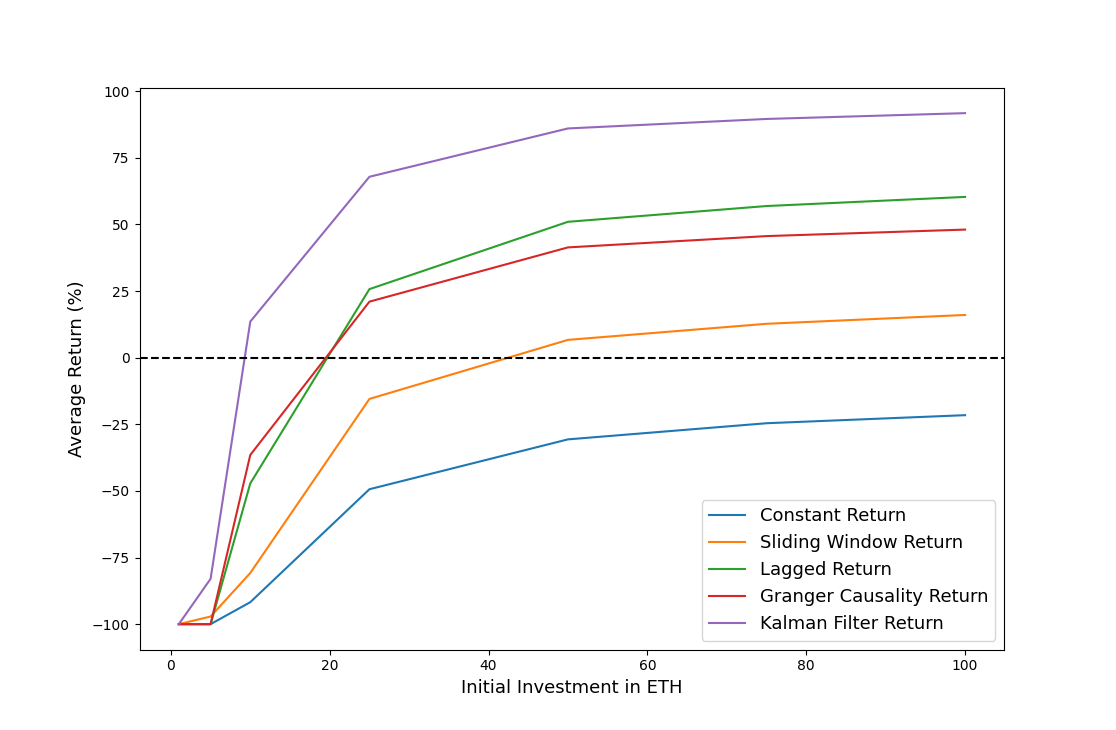
\includegraphics[width=\linewidth]{evaluation/Images/VaryII.png}
    \caption{Average Returns of each strategy using different initial investment volumes}
    \label{fig:VaryInitialInvestments}
\end{figure}

\begin{table}[htb!]
    \centering
    \begin{adjustwidth}{-0.9in}{-0.9in}
        \begin{tabular}{|p{5em}|p{2em}|p{3em}|p{3em}|p{3em}|p{3em}|p{3em}|p{3em}|p{3em}|p{3em}|p{3em}|p{3em}|}\hline
            Initial Investment & Pool Pair & \multicolumn{10}{|c|}{Strategy's Annual Percentage Rate (APR) - Trading from 18th December 2021 to 9th June 2023} \\\cline{3-12}
            &   & \multicolumn{2}{|c|}{Constant} & \multicolumn{2}{|c|}{Sliding Window} & \multicolumn{2}{|c|}{Lagged} & \multicolumn{2}{|c|}{Granger Causality} & \multicolumn{2}{|c|}{Kalman Filter}\\\cline{3-12}
            & & Return \% & \# of Trades & Return \% & \# of Trades & Return \% & \# of Trades & Return \% & \# of Trades & Return \% & \# of Trades\\\hline

            & 0 & \textcolor{red}{-100.0} & 3 & \textcolor{red}{-100.0} & 4 & \textcolor{red}{-100.0} & 2 & \textcolor{red}{-100.0} & 2 & \textcolor{red}{-100.0} & 3\\\cline{3-12}
            & 1 & \textcolor{red}{-100.0} & 3 & \textcolor{red}{-100.0} & 4 & \textcolor{red}{-100.0} & 2 & \textcolor{red}{-100.0} & 2 & \textcolor{red}{-100.0} & 3\\\cline{3-12}
            & 2 & \textcolor{red}{-100.0} & 3 & \textcolor{red}{-100.0} & 4 & \textcolor{red}{-100.0} & 2 & \textcolor{red}{-100.0} & 3 & \textcolor{red}{-100.0} & 3\\\cline{3-12}
            $1 ETH = \$3,946.26$ & 3 & \textcolor{red}{-100.0} & 3 & \textcolor{red}{-100.0} & 4 & \textcolor{red}{-100.0} & 2 & \textcolor{red}{-100.0} & 3 & \textcolor{red}{-100.0} & 3\\[-3ex]\cline{3-12}
            & 4 & \textcolor{red}{-100.0} & 3 & \textcolor{red}{-100.0} & 4 & \textcolor{red}{-100.0} & 2 & \textcolor{red}{-100.0} & 4 & \textcolor{red}{-100.0} & 3\\\cline{3-12}
            & 5 & \textcolor{red}{-100.0} & 3 & \textcolor{red}{-100.0} & 5 & \textcolor{red}{-100.0} & 2 & \textcolor{red}{-100.0} & 2 & \textcolor{red}{-100.0} & 3\\\cline{3-12}
            & 6 & \textcolor{red}{-100.0} & 4 & \textcolor{red}{-100.0} & 3 & \textcolor{red}{-100.0} & 2 & \textcolor{red}{-100.0} & 2 & \textcolor{red}{-100.0} & 2\\\hline\hline
            & 0 & \textcolor{red}{-100.0} & 72 & \textcolor{red}{-100.0} & 133 & \textcolor{red}{-100.0} & 226 & \textcolor{red}{-100.0} & 144 & \textcolor{red}{-92.99} & 146\\\cline{3-12}
            & 1 & \textcolor{red}{-100.0} & 67 & \textcolor{red}{-100.0} & 104 & \textcolor{red}{-100.0} & 162 & \textcolor{red}{-100.0} & 30 & \textcolor{red}{-100.0} & 160\\\cline{3-12}
            & 2 & \textcolor{red}{-100.0} & 79 & \textcolor{red}{-100.0} & 138 & \textcolor{red}{-100.0} & 199 & \textcolor{red}{-100.0} & 132 & \textcolor{red}{-87.15} & 122\\\cline{3-12}
            $5 ETH = \$19,731.30$ & 3 & \textcolor{red}{-100.0} & 71 & \textcolor{red}{-100.0} & 135 & \textcolor{red}{-100.0} & 165 & \textcolor{red}{-100.0} & 112 & \textcolor{red}{-100.0} & 121\\[-3ex]\cline{3-12}
            & 4 & \textcolor{red}{-100.0} & 63 & \textcolor{red}{-100.0} & 135 & \textcolor{red}{-100.0} & 174 & \textcolor{red}{-100.0} & 129 & \textcolor{red}{-88.55} & 139\\\cline{3-12}
            & 5 & \textcolor{red}{-100.0} & 67 & \textcolor{red}{-100.0} & 114 & \textcolor{red}{-100.0} & 147 & \textcolor{red}{-100.0} & 100 & \textcolor{red}{-97.5} & 144\\\cline{3-12}
            & 6 & \textcolor{red}{-100.0} & 37 & \textcolor{red}{-96.31} & 56 & \textcolor{red}{-100.0} & 70 & \textcolor{red}{-100.0} & 8 & \textcolor{red}{-100.0} & 35\\\hline\hline
            & 0 & \textcolor{red}{-100.0} & 241 & \textcolor{red}{-73.29} & 307 & \textcolor{red}{-5.49} & 323 & \textcolor{red}{-9.44} & 176 & \textcolor{green}{28.26} & 146\\\cline{3-12}
            & 1 & \textcolor{red}{-100.0} & 216 & \textcolor{red}{-100.0} & 227 & \textcolor{red}{-100.0} & 291 & \textcolor{red}{-56.99} & 197 & \textcolor{red}{-7.98} & 167\\\cline{3-12}
            & 2 & \textcolor{red}{-72.85} & 201 & \textcolor{red}{-55.37} & 249 & \textcolor{red}{-3.76} & 244 & \textcolor{red}{-1.41} & 161 & \textcolor{green}{28.45} & 122\\\cline{3-12}
            $10 ETH = \$39,462.60$ & 3 & \textcolor{red}{-100.0} & 231 & \textcolor{red}{-100.0} & 240 & \textcolor{red}{-73.99} & 272 & \textcolor{red}{-50.8} & 195 & \textcolor{green}{1.99} & 133\\[-3ex]\cline{3-12}
            & 4 & \textcolor{red}{-80.04} & 217 & \textcolor{red}{-64.22} & 267 & \textcolor{red}{-14.27} & 264 & \textcolor{red}{-11.29} & 187 & \textcolor{green}{30.22} & 139\\\cline{3-12}
            & 5 & \textcolor{red}{-100.0} & 221 & \textcolor{red}{-75.2} & 201 & \textcolor{red}{-48.32} & 226 & \textcolor{red}{-42.44} & 183 & \textcolor{green}{6.61} & 144\\\cline{3-12}
            & 6 & \textcolor{red}{-52.11} & 69 & \textcolor{red}{-37.11} & 56 & \textcolor{red}{-42.18} & 70 & \textcolor{red}{-35.21} & 34 & \textcolor{red}{-30.05} & 67\\\hline\hline

            & 0 & \textcolor{red}{-18.93} & 261 & \textcolor{green}{7.87} & 307 & \textcolor{green}{62.82} & 323 & \textcolor{green}{33.34} & 176 & \textcolor{green}{67.25} & 146\\\cline{3-12}
            & 1 & \textcolor{red}{-71.42} & 336 & \textcolor{red}{-33.85} & 264 & \textcolor{red}{-17.26} & 294 & \textcolor{red}{-5.83} & 197 & \textcolor{green}{28.16} & 167\\\cline{3-12}
            & 2 & \textcolor{red}{-15.96} & 201 & \textcolor{green}{7.51} & 249 & \textcolor{green}{49.6} & 244 & \textcolor{green}{45.58} & 161 & \textcolor{green}{66.77} & 122\\\cline{3-12}
            $25 ETH = \$98,656.50$ & 3 & \textcolor{red}{-58.44} & 287 & \textcolor{red}{-26.86} & 243 & \textcolor{red}{-12.37} & 272 & \textcolor{red}{-3.11} & 195 & \textcolor{green}{32.29} & 133\\[-3ex]\cline{3-12}
            & 4 & \textcolor{red}{-15.09} & 217 & \textcolor{green}{6.05} & 267 & \textcolor{green}{42.03} & 264 & \textcolor{green}{37.49} & 187 & \textcolor{green}{65.93} & 139\\\cline{3-12}
            & 5 & \textcolor{red}{-53.22} & 265 & \textcolor{red}{-19.49} & 201 & \textcolor{green}{2.9} & 226 & \textcolor{green}{4.43} & 183 & \textcolor{green}{40.5} & 144\\\cline{3-12}
            & 6 & \textcolor{red}{-38.19} & 69 & \textcolor{red}{-22.01} & 56 & \textcolor{red}{-26.43} & 70 & \textcolor{red}{-24.02} & 34 & \textcolor{red}{-15.81} & 67\\\hline\hline

            & 0 & \textcolor{red}{-0.76} & 261 & \textcolor{green}{27.61} & 307 & \textcolor{green}{82.45} & 323 & \textcolor{green}{48.52} & 176 & \textcolor{green}{78.51} & 146\\\cline{3-12}
            & 1 & \textcolor{red}{-49.33} & 336 & \textcolor{red}{-16.59} & 264 & \textcolor{red}{-1.54} & 294 & \textcolor{green}{6.43} & 197 & \textcolor{green}{37.68} & 167\\\cline{3-12}
            & 2 & \textcolor{red}{-1.27} & 201 & \textcolor{green}{25.19} & 249 & \textcolor{green}{67.31} & 244 & \textcolor{green}{59.25} & 161 & \textcolor{green}{77.32} & 122\\\cline{3-12}
            $50 ETH = \$197,313.00$ & 3 & \textcolor{red}{-41.96} & 287 & \textcolor{red}{-11.83} & 243 & \textcolor{green}{3.3} & 272 & \textcolor{green}{10.75} & 195 & \textcolor{green}{43.43} & 133\\[-3ex]\cline{3-12}
            & 4 & \textcolor{green}{0.85} & 217 & \textcolor{green}{25.11} & 267 & \textcolor{green}{59.95} & 264 & \textcolor{green}{53.16} & 187 & \textcolor{green}{78.63} & 139\\\cline{3-12}
            & 5 & \textcolor{red}{-37.12} & 265 & \textcolor{red}{-6.58} & 201 & \textcolor{green}{17.6} & 226 & \textcolor{green}{17.37} & 183 & \textcolor{green}{51.84} & 144\\\cline{3-12}
            & 6 & \textcolor{red}{-33.3} & 69 & \textcolor{red}{-17.81} & 56 & \textcolor{red}{-20.8} & 70 & \textcolor{red}{-20.18} & 34 & \textcolor{red}{-11.58} & 67\\\hline\hline

            & 0 & \textcolor{green}{4.54} & 261 & \textcolor{green}{32.75} & 307 & \textcolor{green}{87.19} & 323 & \textcolor{green}{51.42} & 176 & \textcolor{green}{80.97} & 146\\\cline{3-12}
            & 1 & \textcolor{red}{-43.77} & 336 & \textcolor{red}{-12.39} & 264 & \textcolor{green}{2.51} & 294 & \textcolor{green}{9.31} & 197 & \textcolor{green}{39.03} & 167\\\cline{3-12}
            & 2 & \textcolor{green}{2.97} & 201 & \textcolor{green}{29.4} & 249 & \textcolor{green}{70.56} & 244 & \textcolor{green}{61.79} & 161 & \textcolor{green}{79.32} & 122\\\cline{3-12}
            $75 ETH = \$295,969.50$ & 3 & \textcolor{red}{-37.01} & 287 & \textcolor{red}{-8.16} & 243 & \textcolor{green}{6.7} & 272 & \textcolor{green}{13.5} & 195 & \textcolor{green}{45.19} & 133\\[-3ex]\cline{3-12}
            & 4 & \textcolor{green}{6.18} & 217 & \textcolor{green}{29.66} & 267 & \textcolor{green}{64.16} & 264 & \textcolor{green}{56.71} & 187 & \textcolor{green}{81.31} & 139\\\cline{3-12}
            & 5 & \textcolor{red}{-32.1} & 265 & \textcolor{red}{-2.36} & 201 & \textcolor{green}{20.4} & 226 & \textcolor{green}{19.21} & 183 & \textcolor{green}{53.72} & 144\\\cline{3-12}
            & 6 & \textcolor{red}{-31.37} & 69 & \textcolor{red}{-16.19} & 56 & \textcolor{red}{-18.93} & 70 & \textcolor{red}{-18.9} & 34 & \textcolor{red}{-9.98} & 67\\\hline\hline

            & 0 & \textcolor{green}{7.19} & 261 & \textcolor{green}{35.32} & 307 & \textcolor{green}{89.98} & 323 & \textcolor{green}{52.91} & 176 & \textcolor{green}{82.2} & 146\\\cline{3-12}
            & 1 & \textcolor{red}{-40.49} & 336 & \textcolor{red}{-9.77} & 264 & \textcolor{green}{5.2} & 294 & \textcolor{green}{10.93} & 197 & \textcolor{green}{40.46} & 167\\\cline{3-12}
            & 2 & \textcolor{green}{5.12} & 201 & \textcolor{green}{31.92} & 249 & \textcolor{green}{73.17} & 244 & \textcolor{green}{63.31} & 161 & \textcolor{green}{80.48} & 122\\\cline{3-12}
            $100 ETH = \$394,626.00$ & 3 & \textcolor{red}{-34.87} & 287 & \textcolor{red}{-6.13} & 243 & \textcolor{green}{7.72} & 272 & \textcolor{green}{15.23} & 195 & \textcolor{green}{46.48} & 133\\[-3ex]\cline{3-12}
            & 4 & \textcolor{green}{8.38} & 217 & \textcolor{green}{32.28} & 267 & \textcolor{green}{66.24} & 264 & \textcolor{green}{58.31} & 187 & \textcolor{green}{82.52} & 139\\\cline{3-12}
            & 5 & \textcolor{red}{-29.62} & 265 & \textcolor{red}{-0.58} & 201 & \textcolor{green}{22.09} & 226 & \textcolor{green}{20.87} & 183 & \textcolor{green}{55.01} & 144\\\cline{3-12}
            & 6 & \textcolor{red}{-30.43} & 69 & \textcolor{red}{-15.39} & 56 & \textcolor{red}{-18.0} & 70 & \textcolor{red}{-18.27} & 34 & \textcolor{red}{-9.18} & 67\\\hline
        \end{tabular}
    \end{adjustwidth}
    \caption{Returns of each strategy when using different initial investment volumes (Note: Ethereum to USD conversion rate is from 18th December 2021) \label{tab:VaryInitialInvestments}}.
\end{table}

\subsection{Window Size}
The final parameter that also has an effect on the returns is the window size. This window size is used when calculating the mean and standard deviation that are used to calculate the thresholds. As we can see in the excerpt below, the greater the window size, the more data the strategy would use to calculate the thresholds.
\vspace{5mm}
\begin{lstlisting}[language=Python]
spread = self.history_p1[-self.window_size_in_hours:] - self.hedge_ratio * self.history_p2[-self.window_size_in_hours:]
spread_mean = spread.mean()
spread_std = spread.std()
self.upper_threshold = spread_mean + self.number_of_sds_from_mean * spread_std
self.lower_threshold = spread_mean - self.number_of_sds_from_mean * spread_std
\end{lstlisting}
\vspace{5mm}
To evaluate how the window size affects the returns, backtesting is conducted over the period 9th June 2022 to the 9th June 2023, exactly 1 year. The results can be found in Table \ref{tab:VaryWS} and Figure \ref{fig:VaryWS} where we can see that, as the window sizes increase, the returns increase; however, for the smaller window sizes, the return are more erratic and volatile. This volatility decreases as the window size increases, plateauing to each strategy's respective returns.
\\[3mm]
It is also interesting to see that in this period of trading, the Kalman Filter performs the worst, which is surprising as it has outperformed each of the strategies in the experiment that have been previously mentioned.

\begin{figure}[H]
    \centering
    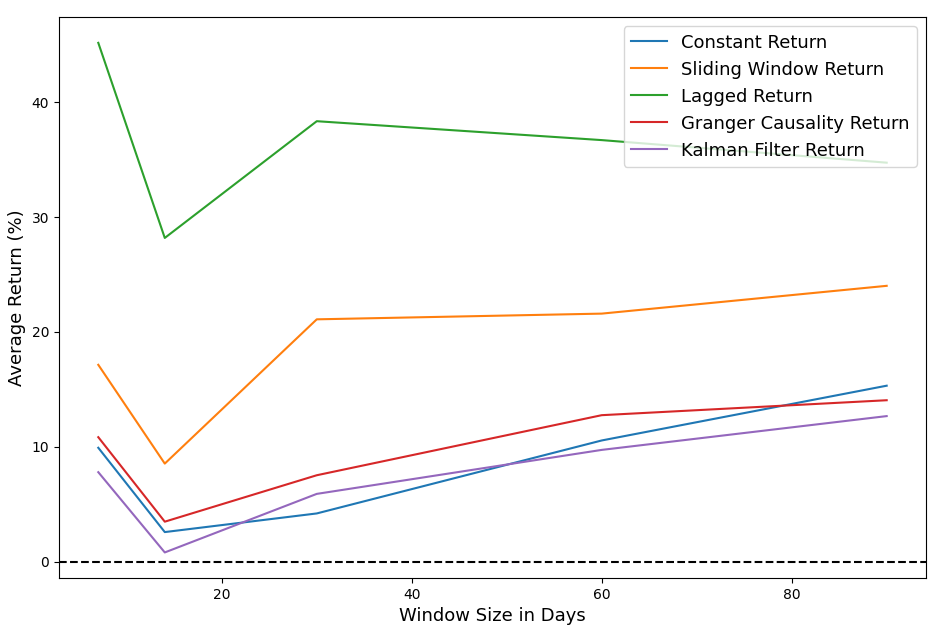
\includegraphics[width=\linewidth]{evaluation/Images/VarWS.png}
    \caption{Average Returns of each strategy using different Window Sizes}
    \label{fig:VaryWS}
\end{figure}

\begin{table}[!htb]
    \centering
    \begin{adjustwidth}{-0.8in}{-0.9in}
        \begin{tabular}{|p{4em}|p{2em}|p{3em}|p{3em}|p{3em}|p{3em}|p{3em}|p{3em}|p{3em}|p{3em}|p{3em}|p{3em}|}\hline
            Window Size & Pool Pair & \multicolumn{10}{|c|}{Strategy's Annual Percentage Rate (APR) - Trading from 9th June 2022 to the 9th June 2023} \\\cline{3-12}
            &   & \multicolumn{2}{|c|}{Constant} & \multicolumn{2}{|c|}{Sliding Window} & \multicolumn{2}{|c|}{Lagged} & \multicolumn{2}{|c|}{Granger Causality} & \multicolumn{2}{|c|}{Kalman Filter}\\\cline{3-12}
            & & Return \% & \# of Trades & Return \% & \# of Trades & Return \% & \# of Trades & Return \% & \# of Trades & Return \% & \# of Trades\\\hline

            & 0 & \textcolor{green}{22.15} & 404 & \textcolor{green}{51.04} & 329 & \textcolor{green}{35.35} & 357 & \textcolor{green}{76.7} & 238 & \textcolor{green}{24.5} & 358\\\cline{3-12}
            & 1 & \textcolor{red}{-36.93} & 328 & \textcolor{red}{-11.1} & 273 & \textcolor{red}{-28.35} & 304 & \textcolor{red}{-1.24} & 316 & \textcolor{red}{-26.28} & 293\\\cline{3-12}
            & 2 & \textcolor{green}{21.97} & 365 & \textcolor{green}{46.2} & 336 & \textcolor{green}{36.53} & 332 & \textcolor{green}{81.15} & 234 & \textcolor{green}{15.32} & 362\\\cline{3-12}
            7 days & 3 & \textcolor{red}{-37.98} & 323 & \textcolor{red}{-18.41} & 278 & \textcolor{red}{-27.55} & 293 & \textcolor{red}{-8.08} & 315 & \textcolor{red}{-35.33} & 306\\\cline{3-12}
            & 4 & \textcolor{green}{26.56} & 377 & \textcolor{green}{44.91} & 351 & \textcolor{green}{40.59} & 344 & \textcolor{green}{83.15} & 255 & \textcolor{green}{23.02} & 334\\\cline{3-12}
            & 5 & \textcolor{red}{-26.07} & 272 & \textcolor{red}{-6.36} & 231 & \textcolor{red}{-21.73} & 249 & \textcolor{green}{15.63} & 268 & \textcolor{red}{-21.63} & 239\\\cline{3-12}
            & 6 & \textcolor{red}{-28.77} & 63 & \textcolor{red}{-21.75} & 67 & \textcolor{red}{-23.42} & 65 & \textcolor{red}{-15.56} & 31 & \textcolor{red}{-27.23} & 67\\\hline\hline

            & 0 & \textcolor{green}{20.66} & 383 & \textcolor{green}{11.37} & 293 & \textcolor{green}{15.97} & 352 & \textcolor{green}{40.32} & 182 & \textcolor{green}{10.84} & 353\\\cline{3-12}
            & 1 & \textcolor{red}{-31.35} & 318 & \textcolor{red}{-24.58} & 249 & \textcolor{red}{-38.7} & 287 & \textcolor{red}{-15.16} & 246 & \textcolor{red}{-34.38} & 277\\\cline{3-12}
            & 2 & \textcolor{green}{17.73} & 327 & \textcolor{green}{10.61} & 283 & \textcolor{green}{5.99} & 311 & \textcolor{green}{38.21} & 186 & \textcolor{green}{6.87} & 311\\\cline{3-12}
            14 days & 3 & \textcolor{red}{-29.1} & 299 & \textcolor{red}{-35.08} & 268 & \textcolor{red}{-40.28} & 297 & \textcolor{red}{-20.64} & 256 & \textcolor{red}{-43.54} & 312\\\cline{3-12}
            & 4 & \textcolor{green}{20.21} & 346 & \textcolor{green}{11.44} & 278 & \textcolor{green}{5.44} & 308 & \textcolor{green}{47.6} & 212 & \textcolor{green}{12.56} & 305\\\cline{3-12}
            & 5 & \textcolor{red}{-18.27} & 251 & \textcolor{red}{-13.4} & 192 & \textcolor{red}{-29.71} & 242 & \textcolor{red}{-8.71} & 200 & \textcolor{red}{-28.11} & 231\\\cline{3-12}
            & 6 & \textcolor{red}{-24.32} & 42 & \textcolor{red}{-17.15} & 45 & \textcolor{red}{-5.46} & 38 & \textcolor{red}{-38.92} & 32 & \textcolor{red}{-19.27} & 45\\\hline\hline

            & 0 & \textcolor{green}{21.69} & 289 & \textcolor{green}{39.05} & 260 & \textcolor{green}{75.61} & 270 & \textcolor{green}{55.53} & 104 & \textcolor{green}{10.56} & 323\\\cline{3-12}
            & 1 & \textcolor{red}{-32.04} & 318 & \textcolor{red}{-9.96} & 219 & \textcolor{red}{-4.39} & 238 & \textcolor{green}{21.46} & 133 & \textcolor{red}{-42.09} & 287\\\cline{3-12}
            & 2 & \textcolor{green}{19.44} & 208 & \textcolor{green}{39.02} & 203 & \textcolor{green}{66.67} & 193 & \textcolor{green}{57.53} & 85 & \textcolor{green}{3.43} & 232\\\cline{3-12}
            30 days & 3 & \textcolor{red}{-26.53} & 274 & \textcolor{red}{-7.43} & 200 & \textcolor{green}{0.83} & 219 & \textcolor{green}{24.28} & 117 & \textcolor{red}{-39.38} & 241\\\cline{3-12}
            & 4 & \textcolor{green}{15.11} & 245 & \textcolor{green}{36.06} & 217 & \textcolor{green}{52.06} & 206 & \textcolor{green}{60.94} & 104 & \textcolor{green}{8.39} & 257\\\cline{3-12}
            & 5 & \textcolor{red}{-12.89} & 214 & \textcolor{green}{2.11} & 153 & \textcolor{green}{14.63} & 168 & \textcolor{green}{35.09} & 105 & \textcolor{red}{-30.14} & 218\\\cline{3-12}
            & 6 & \textcolor{red}{-9.55} & 24 & \textcolor{green}{0.45} & 26 & \textcolor{green}{11.62} & 16 & \textcolor{red}{-23.8} & 21 & \textcolor{red}{-5.29} & 24\\\hline\hline

            & 0 & \textcolor{green}{15.48} & 314 & \textcolor{green}{48.26} & 275 & \textcolor{green}{68.23} & 277 & \textcolor{green}{81.41} & 108 & \textcolor{green}{21.07} & 351\\\cline{3-12}
            & 1 & \textcolor{red}{-28.11} & 303 & \textcolor{red}{-0.49} & 180 & \textcolor{green}{20.55} & 172 & \textcolor{green}{42.31} & 135 & \textcolor{red}{-34.98} & 259\\\cline{3-12}
            & 2 & \textcolor{green}{22.46} & 100 & \textcolor{green}{40.3} & 92 & \textcolor{green}{67.59} & 83 & \textcolor{green}{77.2} & 50 & \textcolor{green}{13.71} & 147\\\cline{3-12}
            60 days & 3 & \textcolor{red}{-6.78} & 179 & \textcolor{green}{13.53} & 112 & \textcolor{green}{39.52} & 96 & \textcolor{green}{56.05} & 68 & \textcolor{red}{-22.18} & 154\\\cline{3-12}
            & 4 & \textcolor{green}{25.22} & 170 & \textcolor{green}{47.69} & 139 & \textcolor{green}{67.06} & 120 & \textcolor{green}{83.31} & 106 & \textcolor{green}{13.68} & 209\\\cline{3-12}
            & 5 & \textcolor{green}{7.16} & 141 & \textcolor{green}{25.9} & 80 & \textcolor{green}{48.05} & 76 & \textcolor{green}{48.54} & 135 & \textcolor{red}{-0.08} & 97\\\cline{3-12}
            & 6 & \textcolor{red}{-7.56} & 23 & \textcolor{green}{2.66} & 25 & \textcolor{green}{14.11} & 15 & \textcolor{red}{-20.72} & 17 & \textcolor{red}{-3.22} & 23\\\hline\hline

            & 0 & \textcolor{green}{16.47} & 238 & \textcolor{green}{47.24} & 289 & \textcolor{green}{64.28} & 295 & \textcolor{green}{87.26} & 71 & \textcolor{green}{30.47} & 287\\\cline{3-12}
            & 1 & \textcolor{red}{-17.53} & 208 & \textcolor{green}{7.99} & 149 & \textcolor{green}{26.87} & 144 & \textcolor{green}{63.9} & 75 & \textcolor{red}{-15.38} & 176\\\cline{3-12}
            & 2 & \textcolor{green}{28.07} & 56 & \textcolor{green}{42.6} & 42 & \textcolor{green}{71.06} & 33 & \textcolor{green}{92.17} & 36 & \textcolor{green}{14.67} & 46\\\cline{3-12}
            90 days & 3 & \textcolor{green}{10.76} & 78 & \textcolor{green}{30.95} & 45 & \textcolor{green}{57.68} & 35 & \textcolor{green}{67.29} & 53 & \textcolor{green}{0.61} & 59\\\cline{3-12}
            & 4 & \textcolor{green}{32.23} & 137 & \textcolor{green}{55.23} & 106 & \textcolor{green}{76.85} & 103 & \textcolor{green}{93.66} & 73 & \textcolor{green}{30.24} & 126\\\cline{3-12}
            & 5 & \textcolor{green}{12.98} & 91 & \textcolor{green}{33.68} & 54 & \textcolor{green}{55.49} & 56 & \textcolor{green}{76.41} & 36 & \textcolor{green}{7.44} & 61\\\cline{3-12}
            & 6 & \textcolor{red}{-7.56} & 23 & \textcolor{green}{2.66} & 25 & \textcolor{green}{14.11} & 15 & \textcolor{red}{-20.72} & 17 & \textcolor{red}{-3.22} & 23\\\hline
            
        \end{tabular}
    \end{adjustwidth}
    \caption{Returns of various Window Sizes \label{tab:VaryWS}}.
\end{table}

\section{Liquidity Pool Pairs Selection}
The choice of liquidity pools have a direct impact on the returns. Immediately, by looking at Section \ref{sec:strat-param}, the selection of liquidity have proven to be successful. However, we could investigate into why these pairs performed particularly well. The main limitation of the pools that could be investigated was that Aave must support both tokens in the liquidity pools and as majority of the token that Aave supports are stablecoins. Therefore, by looking at Table \ref{tab:coin_pools}, it can quickly be seen that all liquidity pairs have some form of a stablecoin aimed to be pegged to the US Dollar. Furthermore, looking at the correlation matrix, Figure \ref{fig:correlationMatrix}, we can immediately see that the pairs associated with tokens pegged to the US Dollar, such as USDT, USDC, and DAI, exhibit the expected high correlation with each other. However, an exception is observed with pool 0xe0554a476a092703abdb3ef35c80e0d76d32939f, which exhibits a lower correlation with other liquidity pools containing these stablecoins. This lower correlation is highly likely due to Uniswap routing swaps via different liquidity pools, causing the price correlation to be lower. Consequently, this lower correlation opens up additional avenues for potential arbitrage opportunities within the pool.

\section{Evaluation of Strategies}
Overall, given the experiments conducted, the optimal parameters for each strategy are different and thus, to evaluate each strategy, Table \ref{tab:OptimParams} displays the optimal parameters used for each strategy.

\begin{table}[H]
    \centering
    \begin{tabular}{|p{6em}|p{8em}|p{6em}|p{4em}|p{8em}|}
    \hline
        Strategy & Number of Standard Deviations from the mean, $\#_{\sigma}$ & Gas Price Threshold in ETH & Window Size in Days & Type of Execution, Seperate or Batched \\ \hline
        Constant & 3 & 6.36e-08 & 60 & Batched \\ \hline
        Sliding Window & 2 & 8.83e-08 & 60 & Batched \\ \hline
        Lagged & 2 & 1.29e-07 & 60 & Batched \\ \hline
        Granger Causality & 1.5 & 2.13e-05 & 60 & Batched \\ \hline
        Kalman Filter & 0.5 & 2.13e-05 & 60 & Batched \\ \hline
    \end{tabular}
    \caption{Optimal Parameters for each strategy \label{tab:OptimParams}}
\end{table}

\noindent By running the backtesting system from 14th January 2022 to 9th June 2023 with an initial investment of 100ETH, we can see in Table \ref{tab:FinalResults} the Kalman Filter outperforms all of the other strategies in all liquidity pool pairs except pair 6. The Granger Causality strategy has also performed well, whereas the Lagged strategy returned mediocre return, with the Constant and the Sliding Window strategies strategy performing similarly, both resulting in around 20\% APY.
\\[3mm]
\begin{table}[H]
    \centering
    \begin{adjustwidth}{-0.8in}{-0.9in}
        \begin{tabular}{|p{4em}|p{3em}|p{3em}|p{3em}|p{3em}|p{3em}|p{3em}|p{3em}|p{3em}|p{3em}|p{3em}|}\hline
            Pool Pair & \multicolumn{10}{|c|}{Strategy's Annual Percentage Rate (APR) - Trading from 14th January 2022 to 9th June 2023} \\\cline{2-11}
            & \multicolumn{2}{|c|}{Constant} & \multicolumn{2}{|c|}{Sliding Window} & \multicolumn{2}{|c|}{Lagged} & \multicolumn{2}{|c|}{Granger Causality} & \multicolumn{2}{|c|}{Kalman Filter}\\\cline{2-11}
            & Return \% & \# of Trades & Return \% & \# of Trades & Return \% & \# of Trades & Return \% & \# of Trades & Return \% & \# of Trades\\\hline
            0 & \textcolor{green}{24.84} & 83 & \textcolor{green}{38.61} & 250 & \textcolor{green}{65.5} & 276 & \textcolor{green}{86.91} & 310 & \textcolor{green}{145.74} & 378\\\cline{2-11}
            1 & \textcolor{green}{20.7} & 37 & \textcolor{green}{14.38} & 127 & \textcolor{green}{29.54} & 151 & \textcolor{green}{20.37} & 269 & \textcolor{green}{43.94} & 456\\\cline{2-11}
            2 & \textcolor{green}{22.12} & 46 & \textcolor{green}{30.74} & 103 & \textcolor{green}{49.75} & 112 & \textcolor{green}{92.19} & 218 & \textcolor{green}{164.55} & 396\\\cline{2-11}
            3 & \textcolor{green}{18.14} & 31 & \textcolor{green}{14.26} & 86 & \textcolor{green}{33.67} & 98 & \textcolor{green}{28.51} & 231 & \textcolor{green}{33.36} & 425\\\cline{2-11}
            4 & \textcolor{green}{27.65} & 45 & \textcolor{green}{38.44} & 122 & \textcolor{green}{66.23} & 140 & \textcolor{green}{92.71} & 290 & \textcolor{green}{152.26} & 391\\\cline{2-11}
            5 & \textcolor{green}{23.11} & 25 & \textcolor{green}{25.76} & 77 & \textcolor{green}{45.57} & 98 & \textcolor{green}{31.8} & 299 & \textcolor{green}{57.81} & 388\\\cline{2-11}
            6 & \textcolor{red}{-2.54} & 13 & \textcolor{red}{-10.28} & 30 & \textcolor{red}{-19.31} & 49 & \textcolor{red}{-10.56} & 23 & \textcolor{red}{-29.71} & 150\\\hline\hline           
            Average & \textcolor{green}{19.14} & 40 & \textcolor{green}{21.70} & 113.6 & \textcolor{green}{38.70} & 132 & \textcolor{green}{48.85} & 234.3 & \textcolor{green}{81.14} & 369.1\\\hline                       
        \end{tabular}
    \end{adjustwidth}
    \caption{Returns of each strategy with their optimal parameters \label{tab:FinalResults}}.
\end{table}

\noindent In addition to this, Figure \ref{fig:ValueHistory} shows the account value over time of each of the strategies; it is easy the see that the account values seem to follow a trend; however, the gradients of the return are less drastic in some strategies, i.e. the Kalman Filter. It is also notable that the number of profitable trades and decreased since the beginning of 2023, with the Kalman Filter strategy taking a large loss in January of this year, 2023.

\begin{figure}[H]
    \centering
    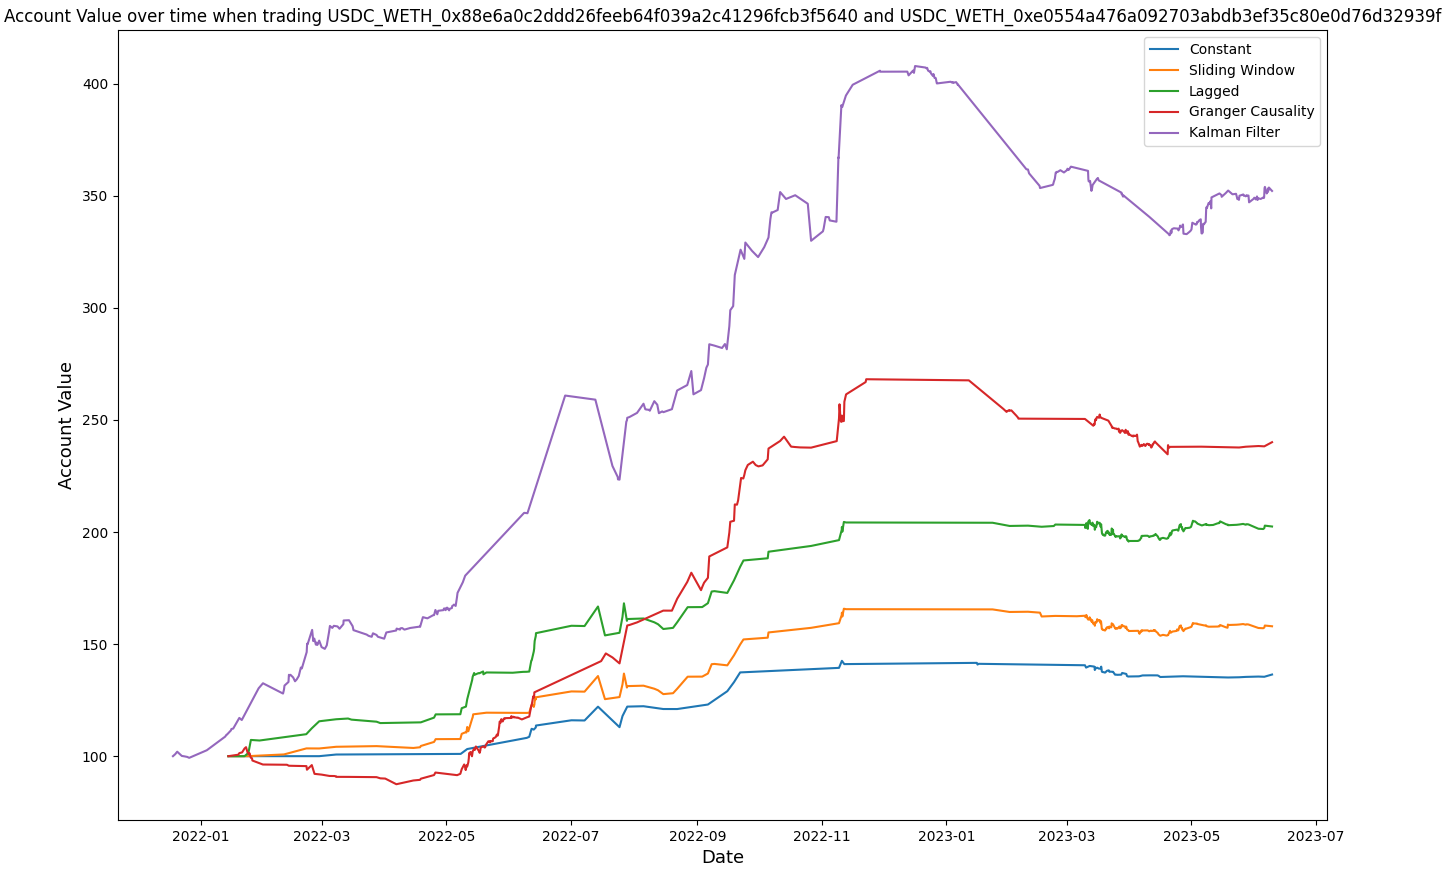
\includegraphics[width=\linewidth]{evaluation/Images/ValueHistory.png}
    \caption{Account Value over Time from backtesting Pair 0}
    \label{fig:ValueHistory}
\end{figure}

\noindent Another valuable insight can be seen in Figure \ref{fig:HedgeRatioPerStrat}, where the evolution of the hedge ratio is plotted for each strategy. It can be seen that the sliding window and the Granger causality strategies' hedge ratios are fairly consistent in comparison to the lagged strategy's hedge ratio. However, the Kalman Filter calculates the Hedge Ratio slightly lower and also more constant with only minor deviations, as can be seen in Figure \ref{fig:evolving_hedge_ratio_kf}. This indicates a more persistent relationship between the paired assets. The minor deviations observed in the hedge ratio can be attributed to temporary fluctuations in market dynamics or noise in the data.

\begin{figure}[H]
    \centering
    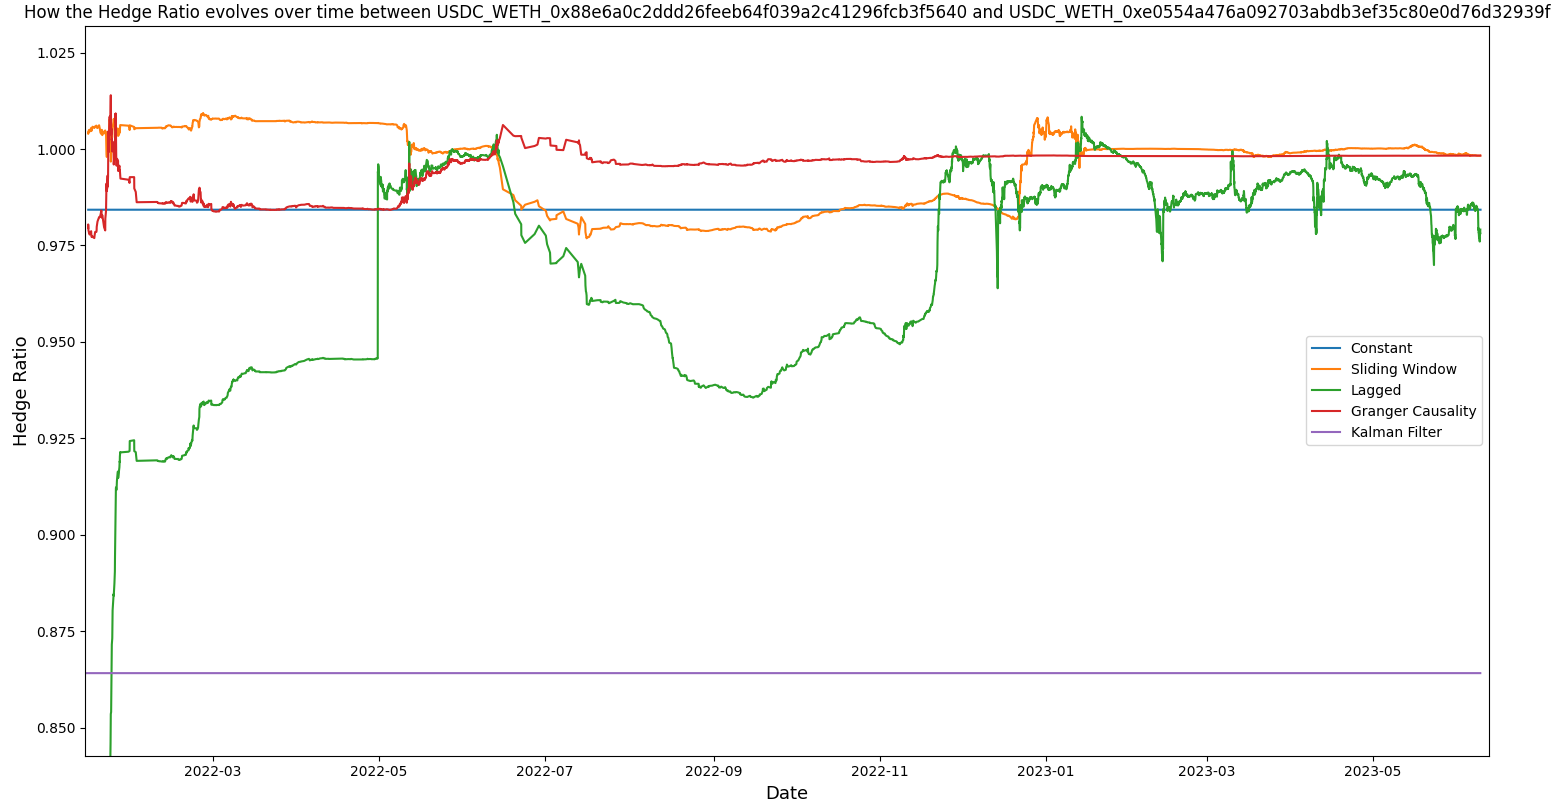
\includegraphics[width=\linewidth]{evaluation/Images/HedgeRatioPerStrat.png}
    \caption{The Hedge Ratio over time for Pair 0}
    \label{fig:HedgeRatioPerStrat}
\end{figure}

\subsection{Beta}
An important metric when evaluating trading strategies or investments that are used in industry is Beta, $\beta$. It measures how correlated the strategy's return is with the market return rate. It is often used as a risk-reward measure, allowing investors to make better decisions when investing, balancing the risk and reward. $\beta$ is defined as $\beta = \frac{Cov(R_M, R_S)}{Var(R_M)}$, where $R_M$ is the market's returns and $R_S$ is the strategy's or stock's returns, the higher the $\beta$ value, the more correlated the strategy's return is with the market whereas a lower one, i.e. $\rightarrow - \infty$, the strategy swings the opposing direction to the market. Therefore, in risk-neutral strategies, a low absolute value is ideal as it minimises the risk.
\\[3mm]
Therefore, to analyse the $\beta$ of each strategy, the conversion from WETH to USD is used as the strategies use WETH as their base currency. As we can see in Table \ref{tab:betas}, the $\beta$s are very close to 0, indicating that the strategy's dependence on the market returns is very low. The low $\beta$ values imply that the trading strategy may be designed to generate returns based on factors other than general market movements. It suggests that the strategy relies more on specific signals, indicators, or market inefficiencies rather than broader market conditions. This can be advantageous in certain situations, as it may allow the strategy to perform well even when the overall market is experiencing volatility or downturns.
\\[3mm]
The comparison of account values and the evolution of ETH price over time are depicted in Figure \ref{fig:beta-vis}. The figure illustrates that there is a limited correlation between the returns of the trading strategy and the price of ETH. While the returns of the strategy do not closely follow the exact movements in the ETH price, it is evident that significant price fluctuations in ETH do have an impact on the strategy's performance. This observation suggests that the trading strategy's returns are influenced, to some extent, by the general trends and movements in the price of ETH. However, it is important to note that the relationship is not entirely linear or directly proportional. Analysing the correlation between the strategy's returns and the price of ETH provides valuable insights into the dynamics of the trading strategy and its sensitivity to market movements. By understanding the impact of ETH price changes on the strategy's performance, traders and investors can make informed decisions and potentially adjust their strategies to optimise their returns and manage risks effectively. It can also be seen that the Constant, Sliding Window and Lagged strategies are less affected by the market compared to the Granger Causality and Kalman Filter strategies.

\begin{table}[H]
    \centering
    \begin{adjustwidth}{-0.8in}{-0.9in}
        \begin{tabular}{|p{5em}|p{7em}|p{7em}|p{7em}|p{8em}|p{7em}|}\hline
            Pool Pair & \multicolumn{5}{|c|}{Strategies' Beta, $\beta$ - Trading from 14th January 2022 to 9th June 2023} \\\cline{1-6}
            & Constant & Sliding Window & Lagged & Granger Causality & Kalman Filter\\\cline{2-6}
            0 & -1.57001e-11 & -2.37822e-11 & -2.34107e-11 & -1.17100e-11 & -3.36017e-11\\\cline{2-6}
            1 & -1.33728e-11 & -2.55276e-11 & -2.34361e-11 & -1.48089e-11 & -2.80161e-11\\\cline{2-6}
            2 & -1.44463e-11 & -2.51260e-11 & -2.48695e-11 & -1.08178e-11 & -3.28074e-11\\\cline{2-6}
            3 & -1.30815e-11 & -2.34876e-11 & -2.48109e-11 & -1.12766e-11 & -3.32465e-11\\\cline{2-6}
            4 & -1.38961e-11 & -2.59124e-11 & -2.78297e-11 & -1.86356e-11 & -3.65904e-11\\\cline{2-6}
            5 & -1.43195e-11 & -3.08987e-11 & -2.79315e-11 & -5.46023e-12 & -3.38610e-11\\\cline{2-6}
            6 & 3.42127e-12 & -4.57712e-11 & -3.56508e-11 & -9.80665e-11 & -1.43624e-10\\\hline\hline
            Average & -1.162784e-11 & -2.864367e-11 & -2.684845e-11 & -2.439650e-11 & -4.882103e-11\\\hline
        \end{tabular}
    \end{adjustwidth}
    \caption{$\beta$s of each strategy \label{tab:betas}}.
\end{table}

\begin{figure}[H]
    \centering
    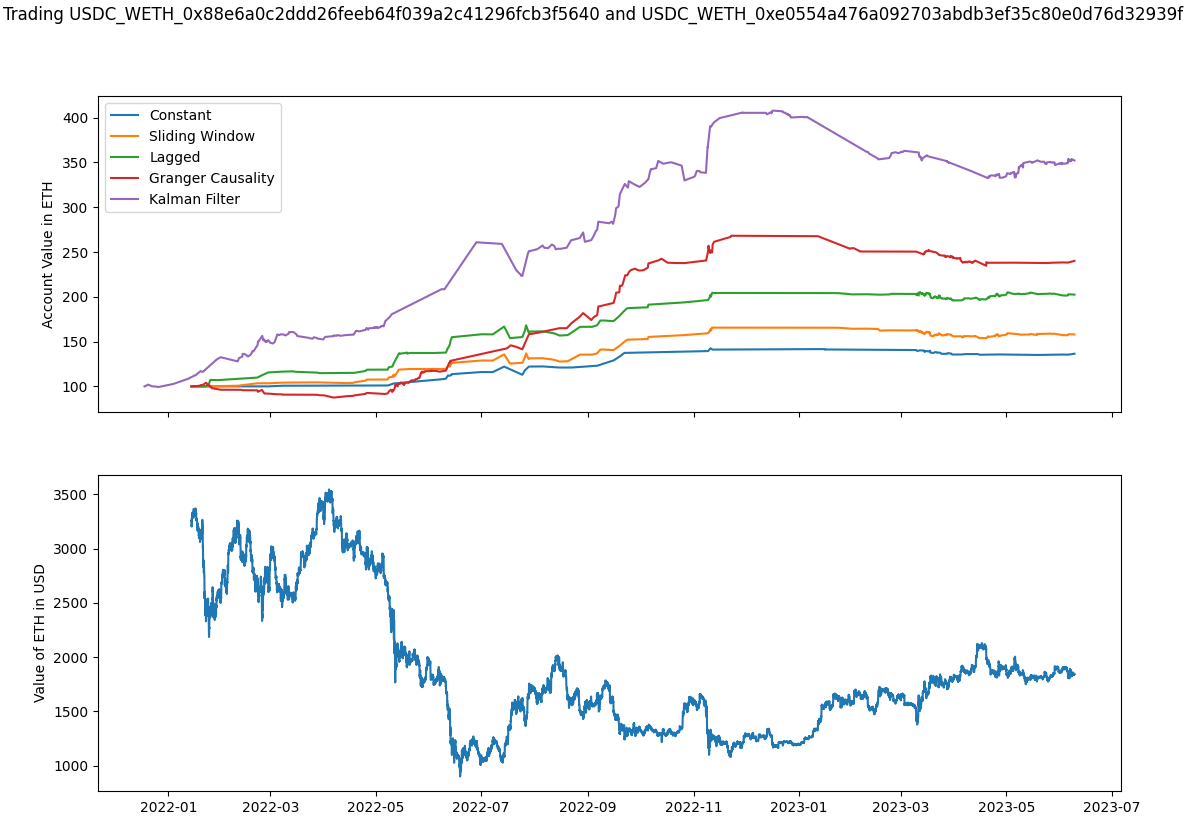
\includegraphics[width=\linewidth]{evaluation/Images/beta_visualisation.png}
    \caption{Account Value of time with the price of ETH}
    \label{fig:beta-vis}
\end{figure}

\subsection{Volatility \& Sharpe Ratio}


Another metric that is commonly used in finance is the Sharpe Ratio; the reason for this is that it is important to evaluate how risky the strategies are compared to the risk-free rate. The metric is given by the formula below:$$\text{Sharpe Ratio} = \frac{R_p - R_f}{\sigma_p}$$ Where $R_p$ is the return of a portfolio, $R_f$ is the risk-free rate and $\sigma_p$ is the standard deviation of the portfolio. A higher Sharpe ratio indicates a better risk-adjusted return, as it signifies a higher return relative to the amount of risk taken. It implies that the investment has achieved a greater excess return compared to the risk-free rate, considering the level of volatility. Conversely, a lower Sharpe ratio suggests a lower risk-adjusted return, indicating a relatively higher level of risk for the given return. The Sharpe ratio also helps investors compare different investments or strategies based on their risk-adversity performance. It provides a way to assess whether the return generated by an investment adequately compensates for the level of risk taken. 
\\[3mm]
To calculate each of the strategies' Sharpe Ratios, the Bank of England's interest rate of 4.5\%~\cite{boe_interest}. Table \ref{tab:sharpes} displays the Sharpe ratios of each strategy; we see that the Constant Strategy exhibits the highest hedge ratio, followed by the Lagged and Granger Causality strategies, while the Sliding Window and Kalman Filter strategies have the lowest Sharpe ratios. This discrepancy can be attributed to the Kalman Filter strategy having a higher variance, indicating a greater level of risk compared to the Sliding Window, Lagged, and Granger Causality strategies. According to Forbes, a Sharpe ratio $>1$ is considered to be `good' as it suggests that the investment or strategy has generated a return that is more than one unit of risk. Overall, all strategies yield desirable Sharpe ratios, indicating favourable risk-adjusted returns.

\begin{table}[H]
    \centering
        \begin{tabular}{|p{7em}|p{7em}|p{7em}|p{7em}|}\hline
            Strategy & Volatility & Average Return & Sharpe Ratio \\\hline
            Constant & 9.28 & 19.14 & 1.46\\\hline
            Sliding Window & 16.02 & 21.70 & 1.10\\\hline
            Lagged & 27.04 & 38.70 & 1.29 \\\hline
            Granger Causality & 38.35 & 48.85 & 1.20\\\hline
            Kalman Filter & 68.34 & 81.14 & 1.17\\\hline
        \end{tabular}
    \caption{Volatility and Sharpe Ratios of each strategy \label{tab:sharpes}}.
\end{table}

\subsection{Comparison with Previous results}
Overall, the strategies seem to be a desirable investment for those with enough capital; however, how do these investments stand against other techniques used? There has not been any research into statistical arbitrage on decentralised exchanges, with the few that have looked into trading in DEXes evaluating pure arbitrage, searching for miss-pricing and executing them. One of which found there to be little to no profitable arbitrage opportunities on various decentralised exchanges, including Uniswap, regardless of volume size~\cite{boonpeam2021arbitrage}. This happens as the pair prices as automatically adjusted based on supply and demand, making the opportunities limited, short-lived and costly. In comparison, the results from the strategies implemented in this paper do generate a profit in comparison to the cyclic arbitrage approach.
\\[3mm]
Other research into statistical approaches to arbitrage has been done on more mainstream assets such as ETFs; however, they have not been experimented on cryptocurrencies. One paper used the Kalman Filter on ETFs and ETNs and found there to be an average of 25.17\% returns in 1 year in in-sample backtesting; however, it failed to generate any profit in its out-of-sample results~\cite{dempsey_market_2017}. The implemented Lagged, Kalman Filter, and Granger Causality trading strategies yield a greater APR compared to this. In addition to this, another piece of research used a combination of machine learning and the Kalman Filter on assets on the BM\&FBovespa Exchange, yielding a return of 26.13\% in the out-of-sample results~\cite{6974093}. In comparison, the Lagged, Kalman Filter and Granger Causality strategies implemented in this paper have a greater return; however, the strategy implemented by Oliveira and Nóbrega, possesses a greater Sharpe ratio meaning the risk-adjusted returns are more favourable. To summarise, three of the five strategies implemented outperform the current research out there on both purer forms of arbitrage, i.e. cyclic arbitrage, and also the use of Kalman Filter on other types of assets, i.e. ETFs and ETNs.
